% !TEX root = ../22830110_dissertation.tex
\chapter{Methodology}
\label{chap:methodology}

\section{Introduction}
This chapter outlines the methodological framework used to design, build, and evaluate the AI-driven financial note generation system. It begins with the underlying architecture of modern Large Language Models (LLMs), in particular the Transformer. It then sets out the deployment infrastructure, the multi-agent architecture implemented with CrewAI, and the benchmarking framework used to compare the GPT-5.4 prompting baseline with the callable GPT-4.1 fine-tuned deployments produced from the project training recipes.

\section{Deep Dive: The Architecture of Transformers}
Prior to 2017, the dominant architectures for Natural Language Processing (NLP) were Recurrent Neural Networks (RNNs) and their more advanced variant, Long Short-Term Memory (LSTM) networks. While effective for short sequences, these models processed data sequentially, which inherently limited their ability to scale across parallel hardware and often caused them to "forget" earlier context in long documents. 

The publication of "Attention Is All You Need" by Vaswani et al. (2017) introduced the Transformer, an architecture that dispensed entirely with recurrence and convolutions in favor of an "attention" mechanism. This paradigm shift forms the foundational technology for all modern LLMs, including the ones used in this research.

\subsection{Self-Attention Mechanism}
At the core of the Transformer is the self-attention mechanism, which allows the model to determine the relevance of all other words in a sequence when encoding a specific word. In the context of financial accounting, this means the model can dynamically link a referenced "accrual" on page five to the specific "invoice date" mentioned on page one.

The mechanism operates by mapping a query and a set of key-value pairs to an output. For each word (token) in the input, three vectors are created through learned linear transformations: a Query vector (\$Q\$), a Key vector (\$K\$), and a Value vector (\$V\$). 

The attention score is computed using the scaled dot-product attention formula:
\begin{equation}
\text{Attention}(Q, K, V) = \text{softmax}\left(\frac{QK^T}{\sqrt{d_k}}\right)V
\end{equation}
where $d_k$ is the dimension of the key vectors. The dot product of the query with all keys dictates the weight (or focus) placed on each corresponding value. The division by $\sqrt{d_k}$ serves to scale the gradients, preventing them from vanishing or exploding during training.

\subsection{Multi-Head Attention and Positional Encoding}
Rather than performing a single attention function, Transformers use "Multi-Head Attention." This allows the model to jointly attend to information from different representation subspaces at different positions. For instance, one "head" might learn to attend to grammatical structure, while another attends to numeric relationships—a critical feature when parsing a Trial Balance.

Because the Transformer processes all tokens simultaneously, it lacks inherent knowledge of word order. To rectify this, positional encodings are added to the input embeddings at the bottoms of the encoder and decoder stacks. These encodings inject information about the relative or absolute position of the tokens in the sequence, using sine and cosine functions of different frequencies.

\subsection{Encoder vs. Decoder Architectures}
The original Transformer featured both an encoder (to map the input to a continuous representation) and a decoder (to generate the output sequence). Subsequent architectures diverged based on their use cases:
\begin{itemize}
    \item \textbf{Encoder-Only (e.g., BERT):} Excellent for tasks requiring deep bidirectional understanding, such as sentiment analysis or named entity recognition.
    \item \textbf{Decoder-Only (e.g., GPT series):} Optimised for autoregressive text generation. These models predict the next token based on all previous tokens, making them ideal for generating the narrative of a year-end accounting note.
\end{itemize}

\begin{figure}[H]
    \centering
    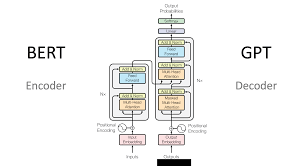
\includegraphics[width=0.75\textwidth]{figures/transformer-model}
    \caption{The Original Transformer Architecture (Vaswani et al., 2017)}
    \label{fig:transformer_model}
\end{figure}

\section{AI Infrastructure for Production}
The deployment of these complex architectures requires sophisticated infrastructure. The shift from localized CPU processing to distributed GPU clusters has been pivotal. 

\subsection{Compute and Cloud Deployment}
Modern LLMs, containing billions or trillions of parameters, require immense parallel compute power provided by GPUs (e.g., NVIDIA H100s). For an enterprise financial application, hosting these models locally is often cost-prohibitive. Thus, this project leverages cloud-based API endpoints, specifically Azure OpenAI, which provides enterprise-grade security, scalability, and adherence to data privacy regulations (UK GDPR).

\begin{figure}[H]
    \centering
    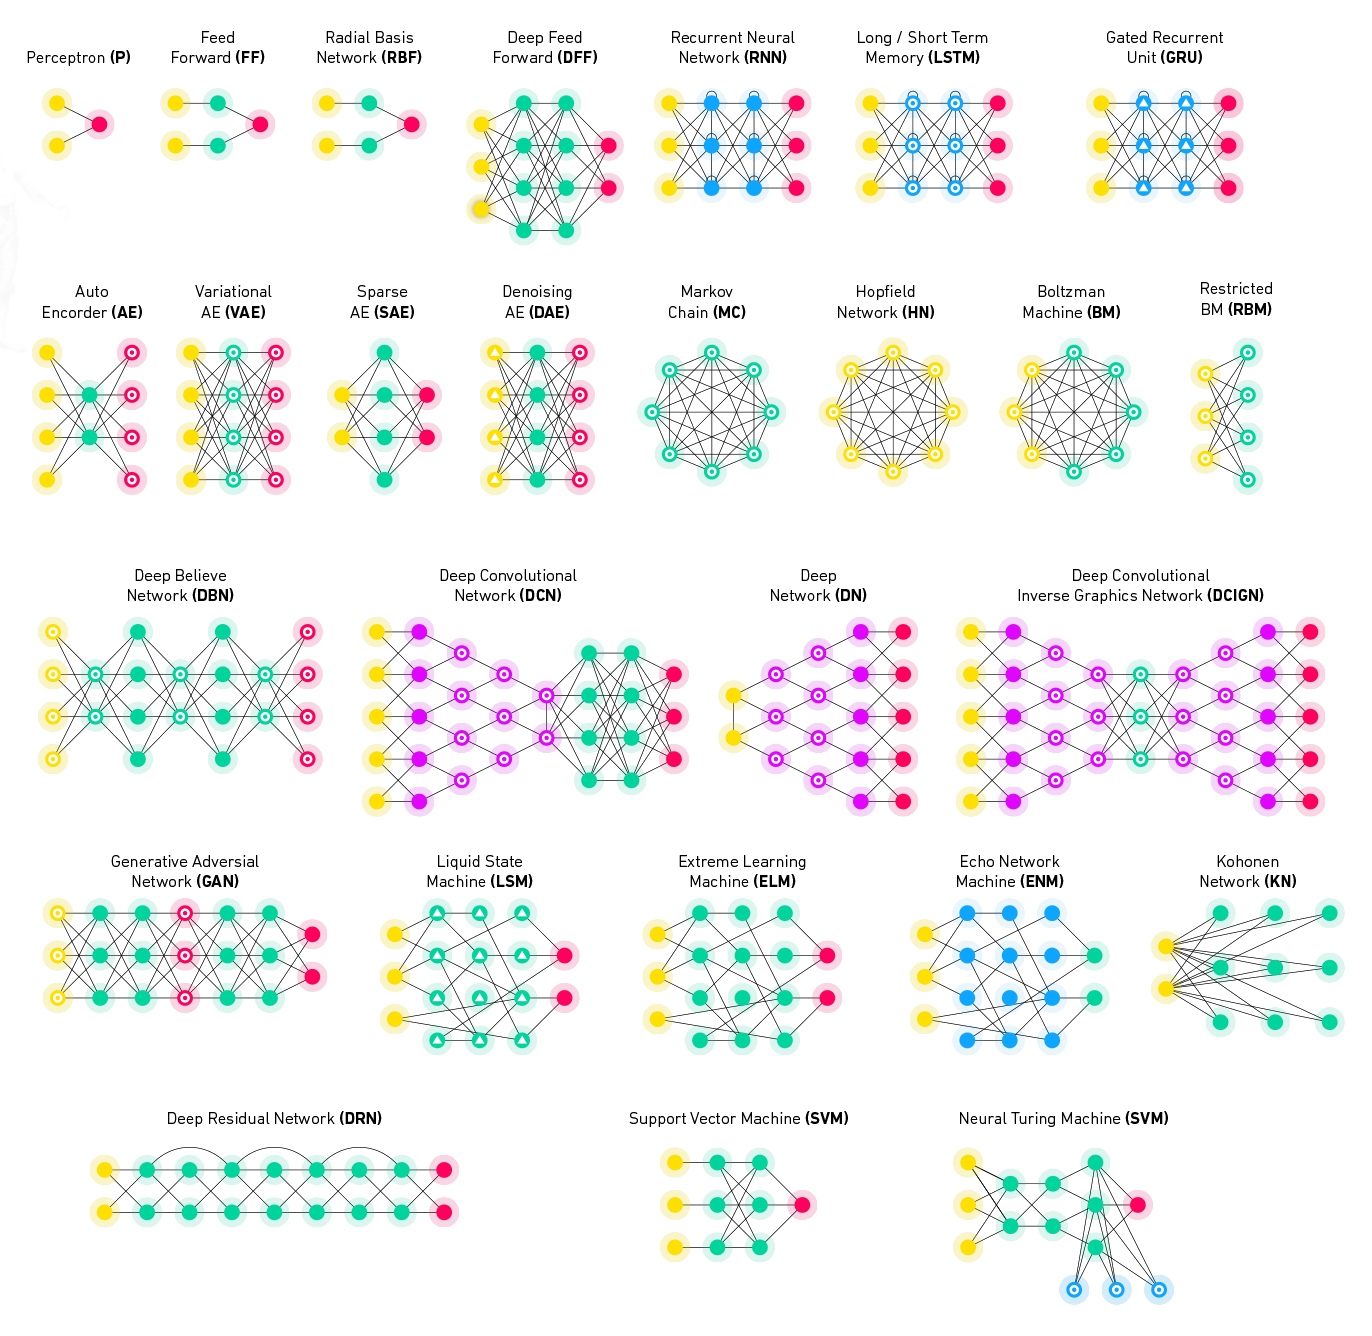
\includegraphics[width=0.8\textwidth]{figures/different_ai_models}
    \caption{Landscape of Modern AI Models and Cloud Providers}
    \label{fig:different_ai_models}
\end{figure}

\subsection{Vector Databases and Embeddings}
To prevent the model from generating plausible but incorrect financial data—a phenomenon known as "hallucination"—the infrastructure integrates Retrieval-Augmented Generation (RAG). RAG utilizes Vector Databases (such as Pinecone or ChromaDB). Documents, accounting standards, and historical client ledgers are converted into high-dimensional vector embeddings. When the AI requires context, the system performs a cosine-similarity search across the vector database to retrieve the mathematically closest factual documents, appending them to the LLM's prompt. This significantly grounds the model's responses in factual reality.

\section{The System Architecture: Multi-Agentic Framework}
While a single LLM prompt can generate text, an audit-ready financial system requires rigorous checks and balances. This dissertation implements a multi-agentic framework using CrewAI. Rather than relying on a monolithic assistant, the architecture decomposes the workload into distinct, specialised roles mimicking a real-world accounting firm.

\begin{enumerate}
    \item \textbf{Senior Financial Analyst (Data Extraction):} This agent operates purely deterministically. Following the "Decimal Mandate," it extracts raw data from the Xero API, refusing to use floating-point arithmetic. It isolates variances greater than 10\% and formats the structured JSON payload.
    \item \textbf{Accounting Partner (Narrative Writer):} This LLM-powered agent receives the deterministic payload and is tasked with synthesizing the human-readable narrative. It is strictly prompted to use the "You" perspective and adhere to statutory narrative sequencing (Turnover, Corporation Tax, Balance Sheet).
    \item \textbf{Quality Control Reviewer (Compliance Assessor):} The final agent reviews the generated text against a strict set of rules (e.g., no explicit journal numbers in the text, verification of numeric matching against the JSON payload). If discrepancies are found, a \textit{ReconciliationError} is raised, and the text is sent back to the Writer for correction.
\end{enumerate}

\subsection{Illustrative Methodology Example}
One representative validation case involves a technology company with unresolved equity movements. In the source working papers, the main issue was whether the year-end note should state a final position on share capital and share premium before the supporting paperwork had been completed. A generic prompting workflow could easily turn the visible movement in equity into a confident summary.

The deterministic layer first identifies investment-related balances and legal or professional-fee activity. The writer agent then drafts a narrative from those facts, while the reviewer agent checks that the wording does not overstate certainty. In the validation corpus, one accountant-authored gold note states that the team is still waiting for investment and share issue confirmation before finalising the share capital and share premium figures. This example shows that accuracy in accounting narrative depends on more than numeric agreement. It also depends on retaining uncertainty where the evidence is incomplete. That point shaped both the fine-tuning dataset and the evaluation rubric used later in the dissertation.

\begin{figure}[H]
    \centering
    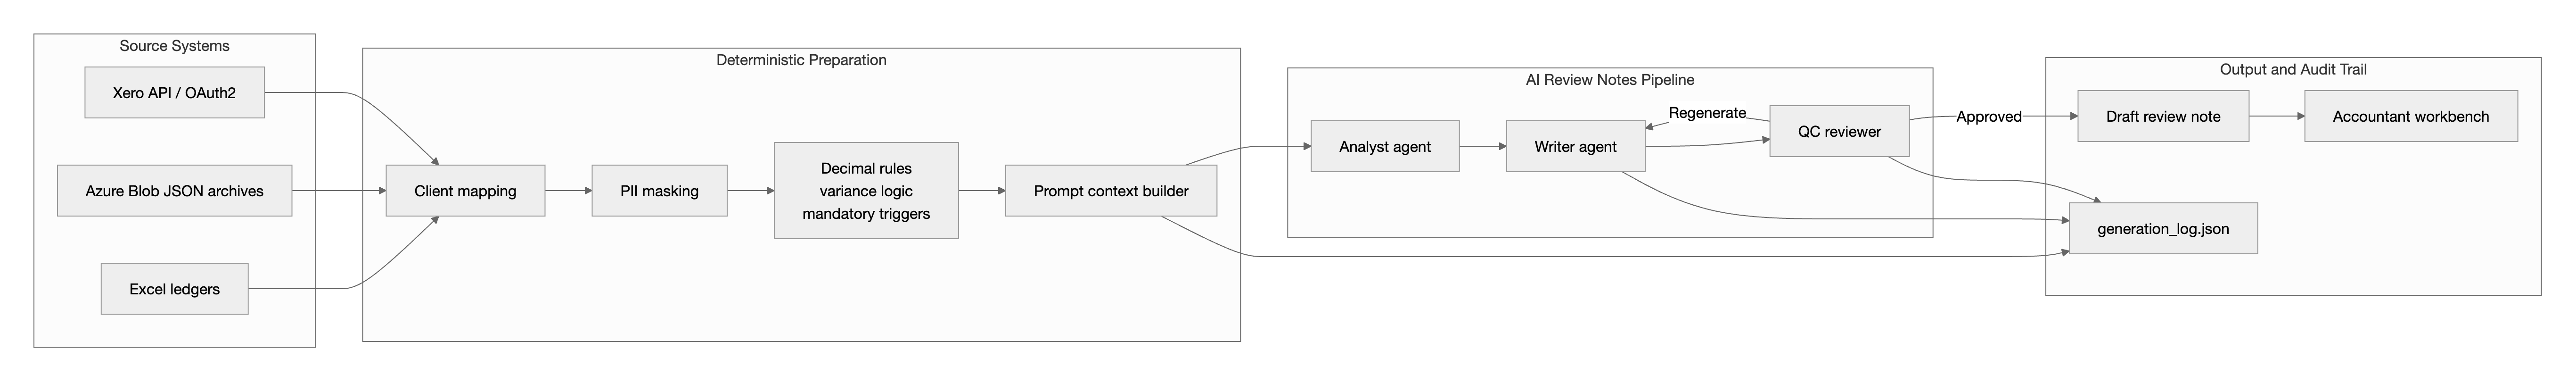
\includegraphics[width=0.92\textwidth]{figures/architecture_diagram}
    \caption{End-to-End System Architecture for the AI Review Notes Pipeline}
    \label{fig:architecture_diagram}
\end{figure}

\section{UX/UI Design and Development}
The effectiveness of an AI-driven system is not solely dependent on its algorithmic performance; the user interface (UI) and user experience (UX) play a critical role in how financial professionals interact with and trust the AI's output. For the PHM UK application, a bespoke design system was developed to ensure clarity, security, and precision.

\subsection{Design Philosophy: Authority, Precision, and Trust}
The design language is anchored in three core pillars:
\begin{itemize}
    \item \textbf{Authority:} A palette of deep navy tones establishes a sense of institutional stability and professional reliability.
    \item \textbf{Precision:} A disciplined 8px grid system and sharp typography (Inter) ensure that dense financial data is presented with mathematical rigor.
    \item \textbf{Trust:} The interface avoids aggressive visual elements, using ambient shadows and high whitespace to focus the accountant's attention on the AI-generated notes and their source data.
\end{itemize}

\subsection{User Journey and Wireframe Development}
To validate the UX, a series of low-fidelity wireframes and high-fidelity interface screens were developed representing the primary accountant journey. The wireframes establish the functional layout, review flow, and feedback loop before the visual layer is applied.

\begin{figure}[H]
    \centering
    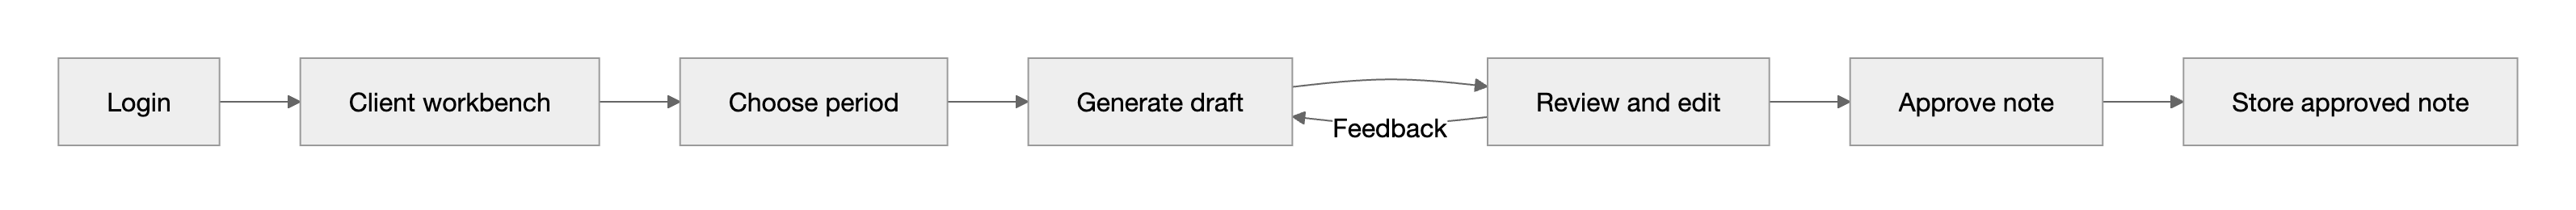
\includegraphics[width=0.88\textwidth]{figures/ui_flow_diagram}
    \caption{Primary User Journey from Authentication to Approved Review Note}
    \label{fig:ui_flow_diagram}
\end{figure}

\begin{figure}[H]
    \centering
    \begin{subfigure}[b]{0.48\textwidth}
        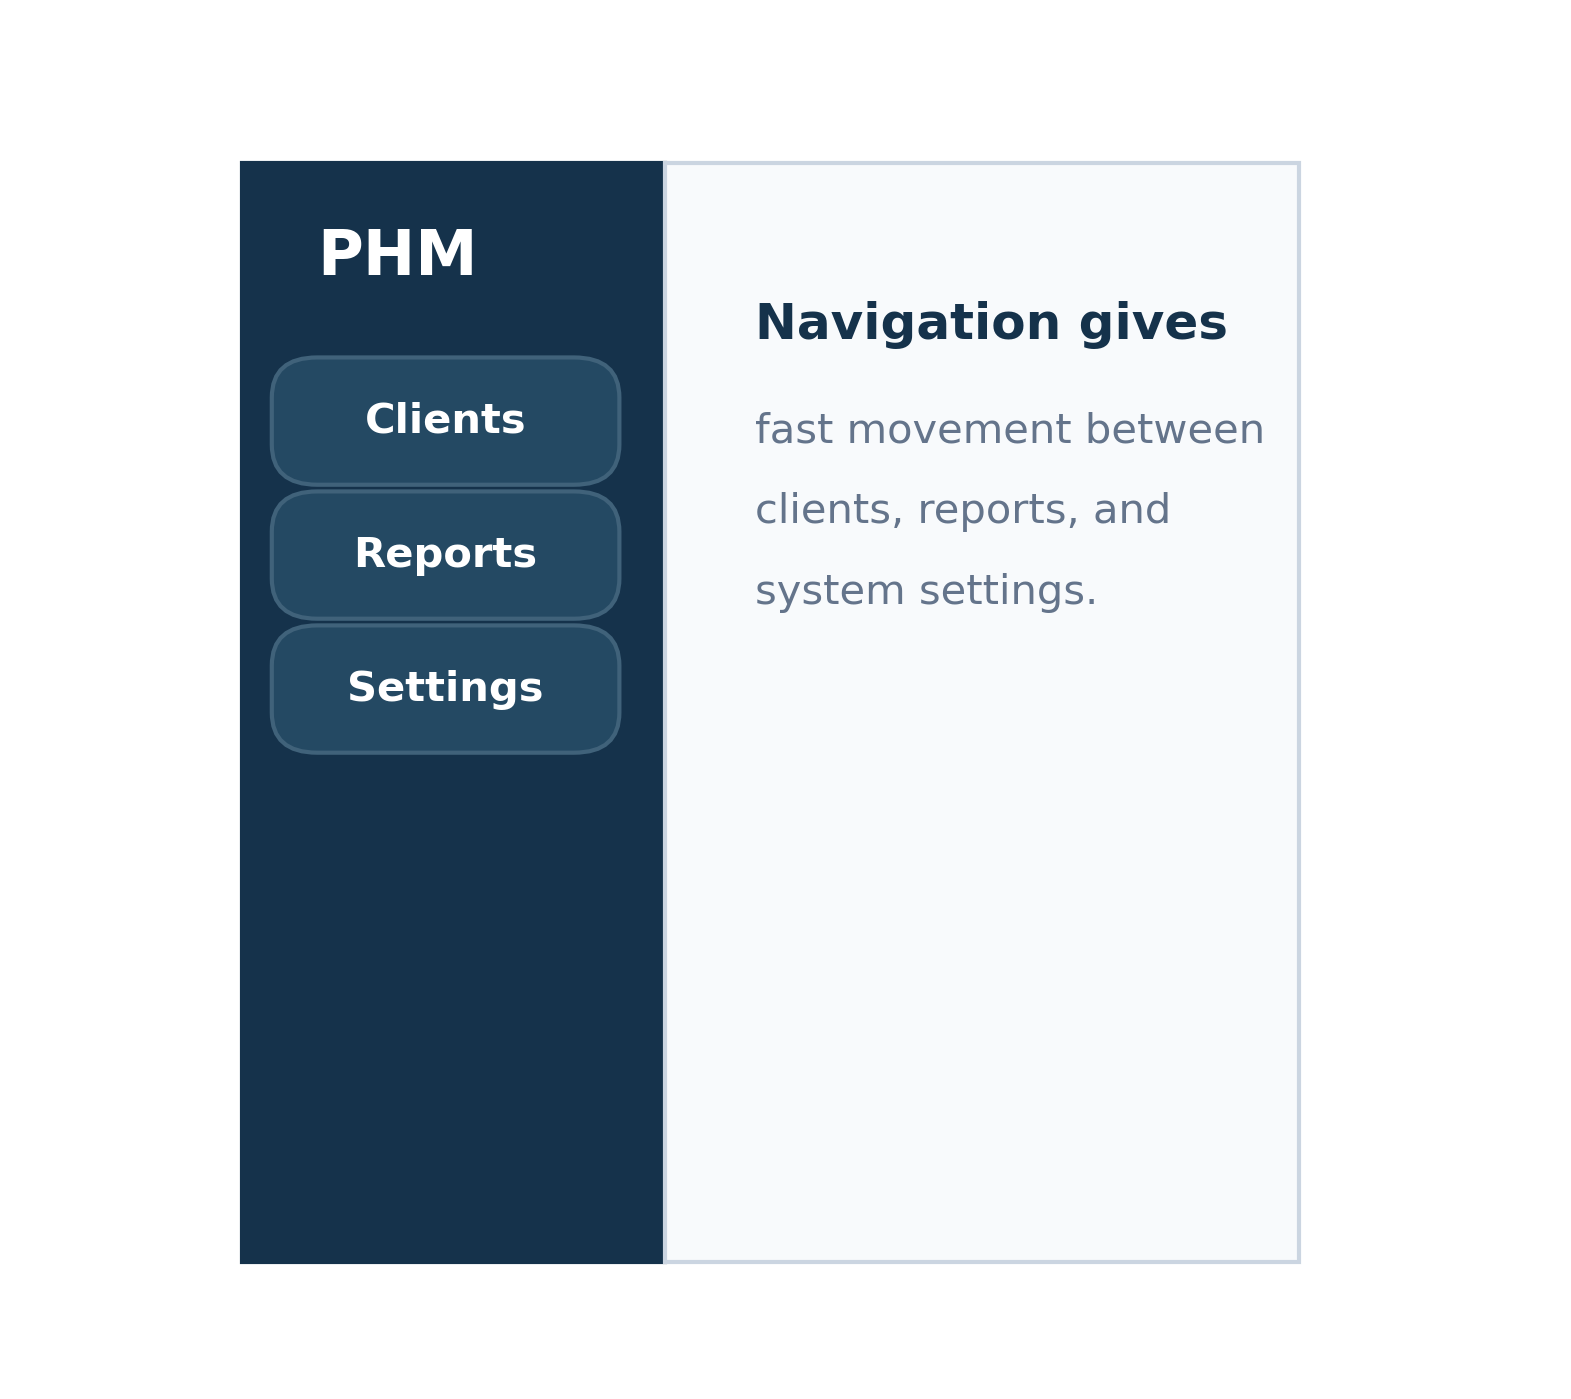
\includegraphics[width=\textwidth]{figures/sidebar_wireframe}
        \caption{Sidebar Navigation Model}
    \end{subfigure}
    \hfill
    \begin{subfigure}[b]{0.48\textwidth}
        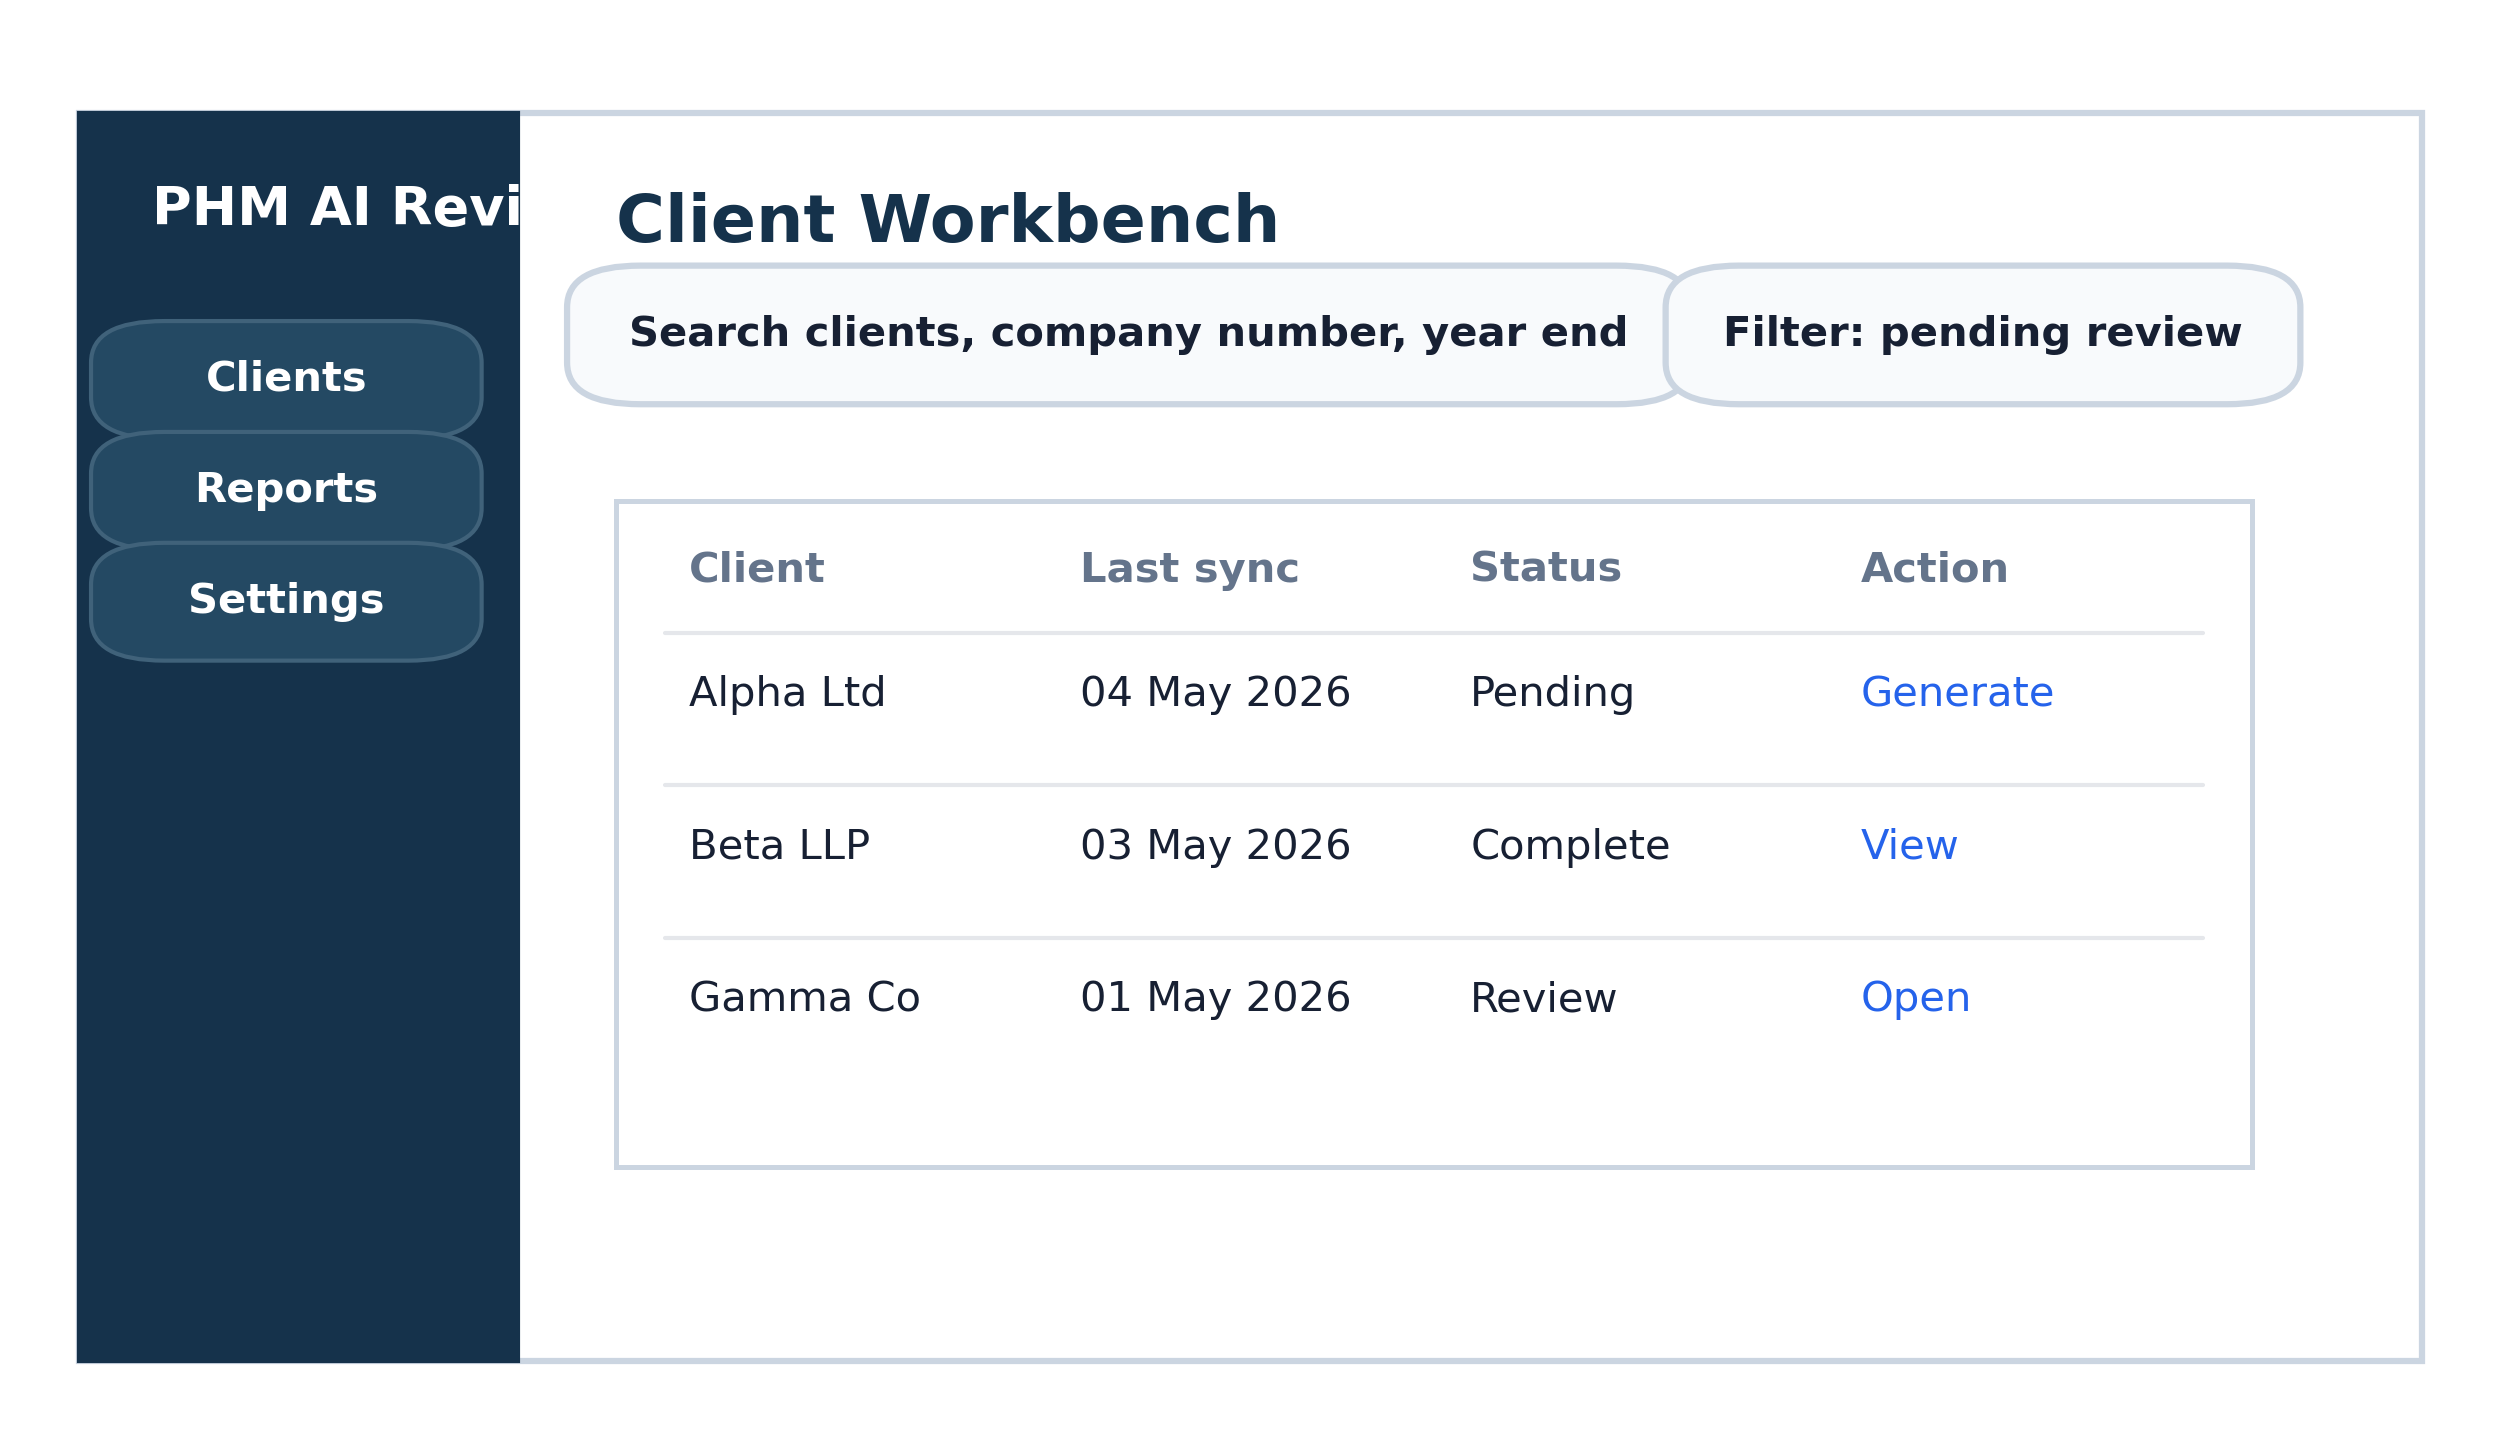
\includegraphics[width=\textwidth]{figures/dashboard_wireframe}
        \caption{Client Workbench Wireframe}
    \end{subfigure}
    \caption{Low-Fidelity Navigation and Dashboard Wireframes}
    \label{fig:navigation_dashboard_wireframes}
\end{figure}

\begin{figure}[H]
    \centering
    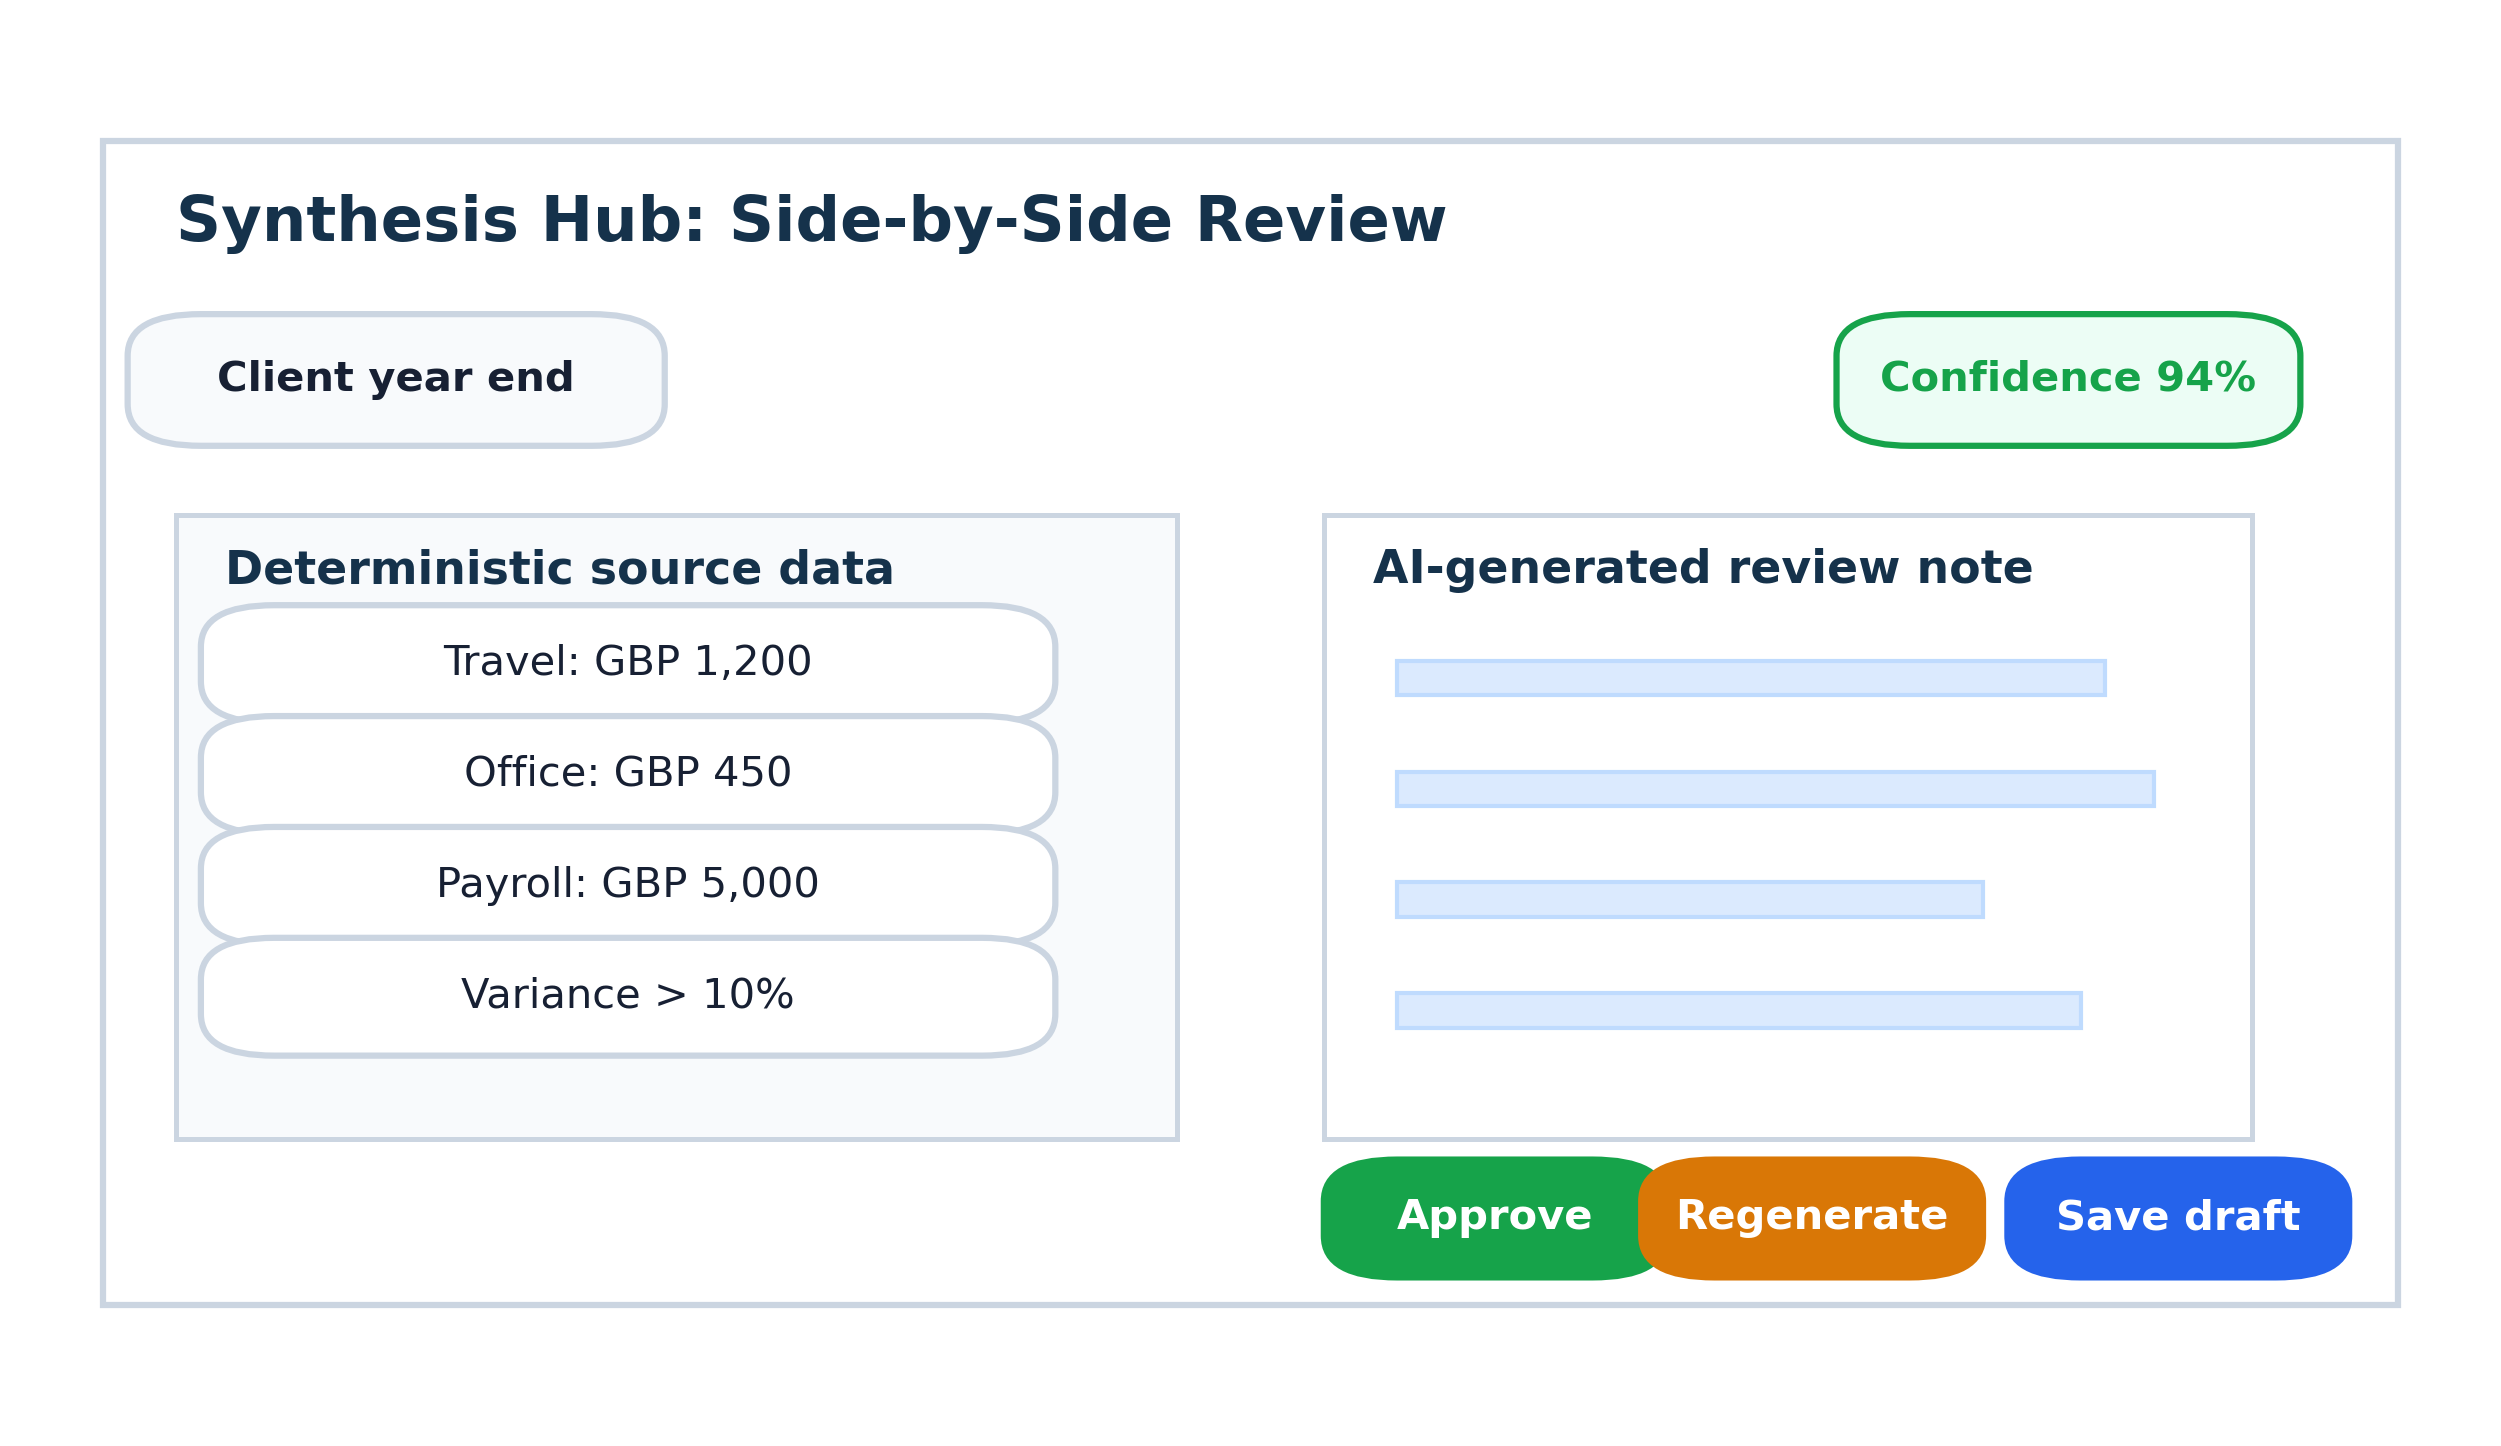
\includegraphics[width=0.9\textwidth]{figures/review_wireframe}
    \caption{Low-Fidelity Side-by-Side Review Wireframe}
    \label{fig:review_wireframe}
\end{figure}

The following high-fidelity screens show the same journey translated into the implemented Flask interface.

\begin{figure}[H]
    \centering
    
\includegraphics[width=0.7\textwidth]{figures/LOGIN PAGE}
    \caption{User Authentication Interface (Login Page)}
    \label{fig:login_page}
\end{figure}

\begin{figure}[H]
    \centering
    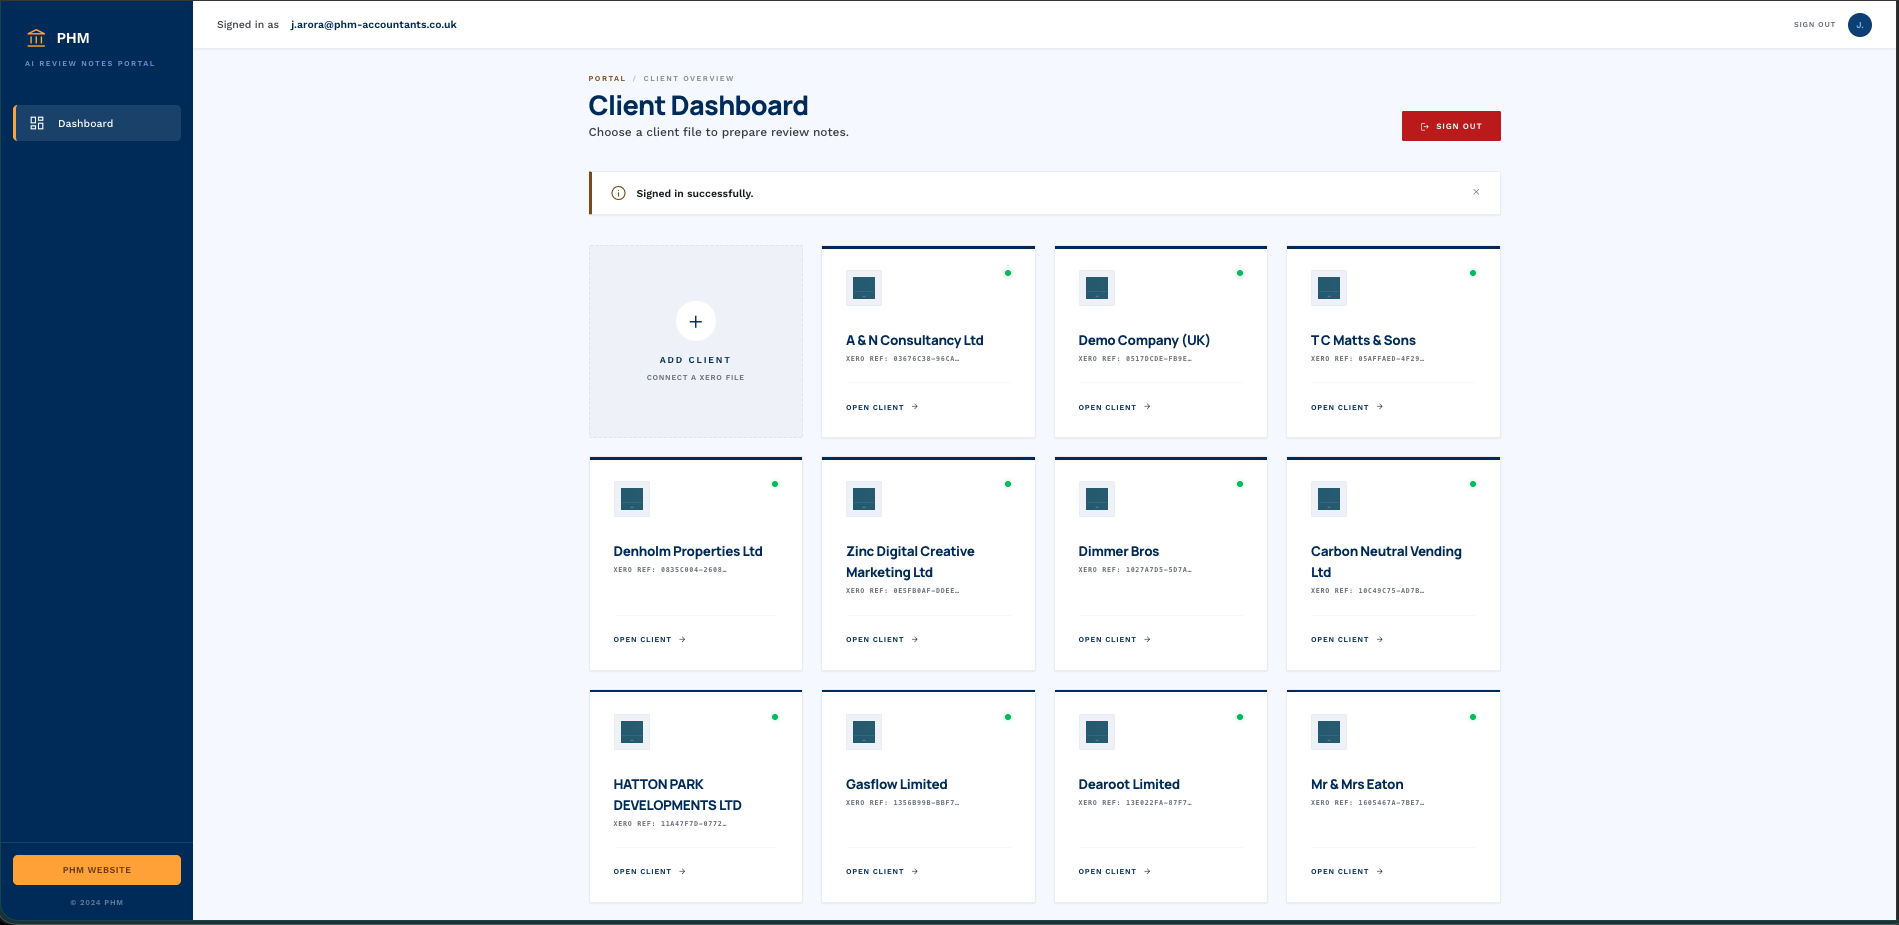
\includegraphics[width=0.9\textwidth]{figures/CLIENTS PAGE}
    \caption{Accountant Workbench: Client Portfolio Overview}
    \label{fig:clients_page}
\end{figure}

\begin{figure}[H]
    \centering
    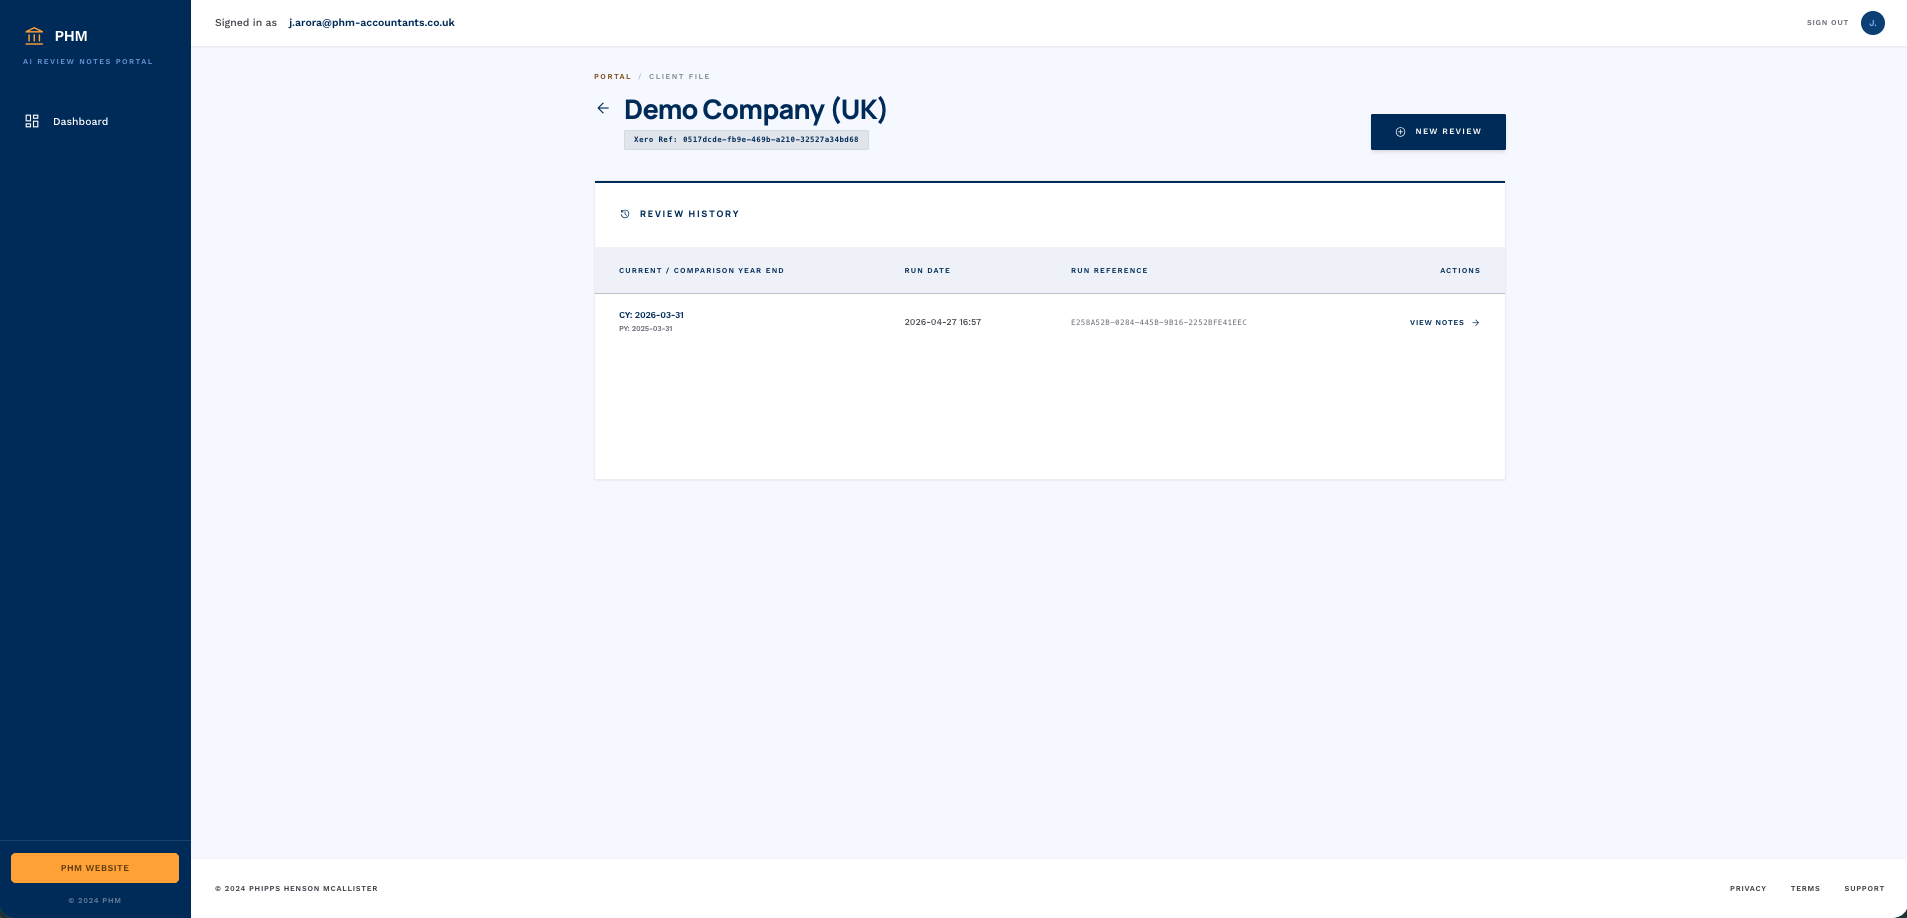
\includegraphics[width=0.9\textwidth]{figures/REPORTS PAGE}
    \caption{Synthesis Hub: Review and Approval Panel}
    \label{fig:reports_page}
\end{figure}

\begin{figure}[H]
    \centering
    \begin{subfigure}[b]{0.45\textwidth}
        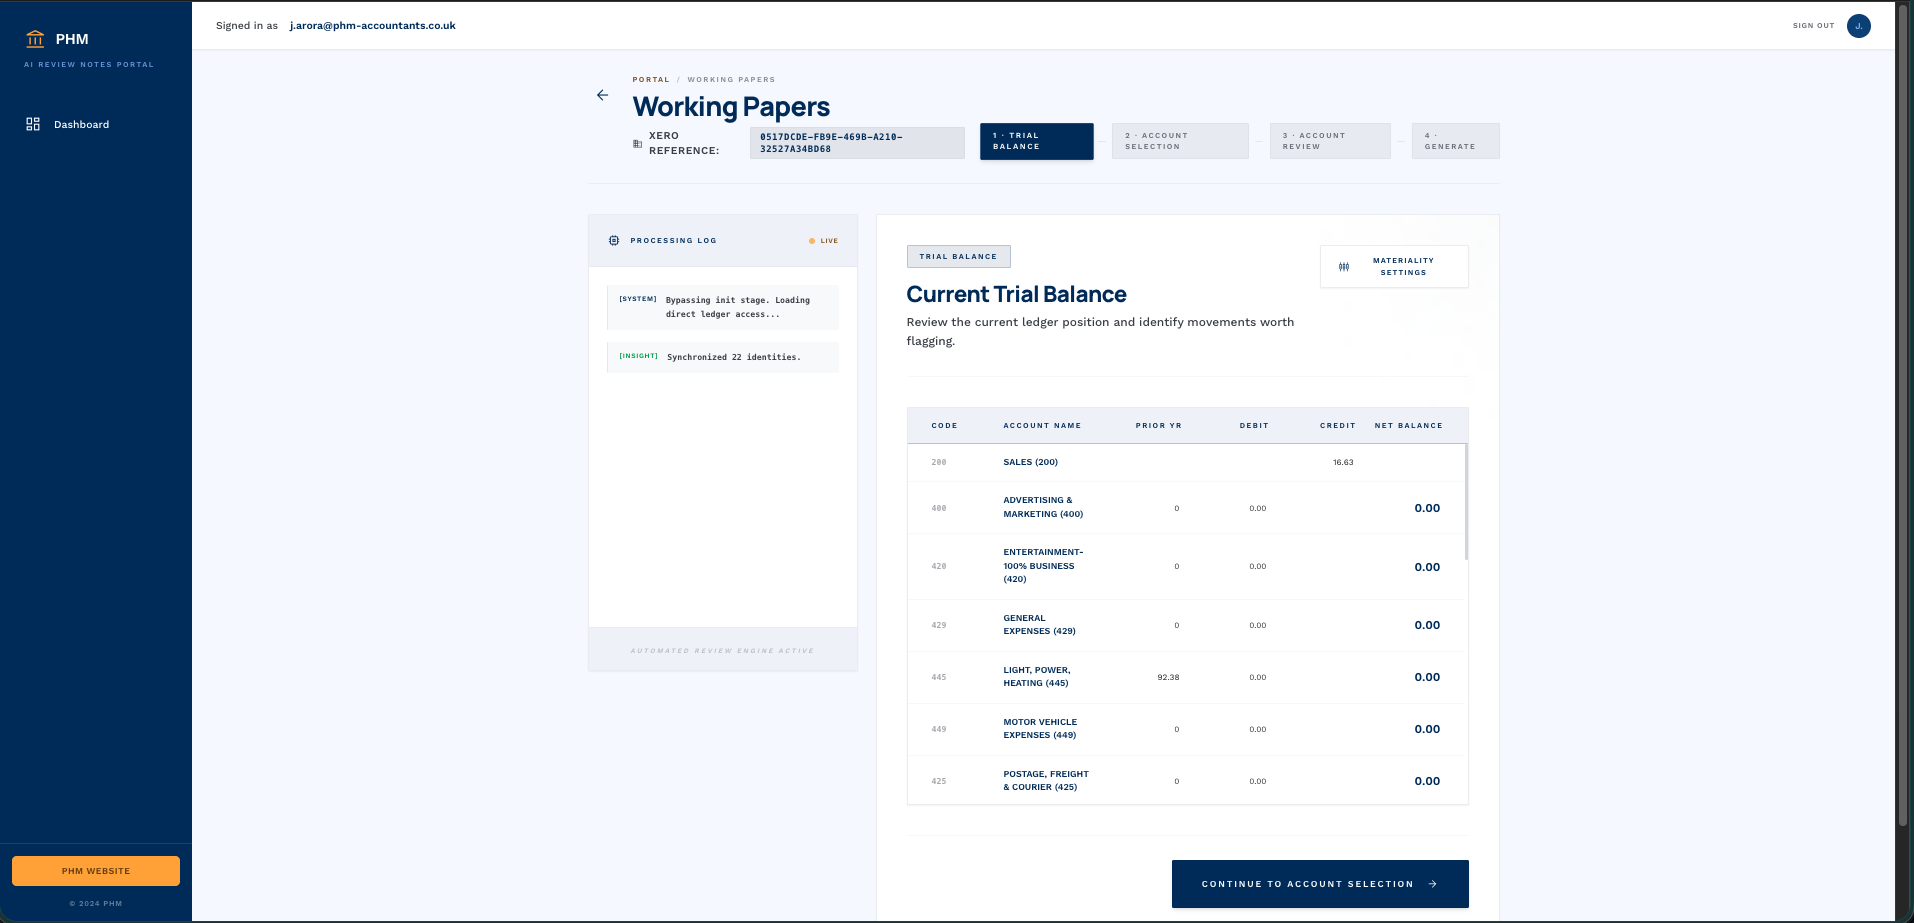
\includegraphics[width=\textwidth]{figures/INIT PAGE}
        \caption{Initial Generation State}
    \end{subfigure}
    \hfill
    \begin{subfigure}[b]{0.45\textwidth}
        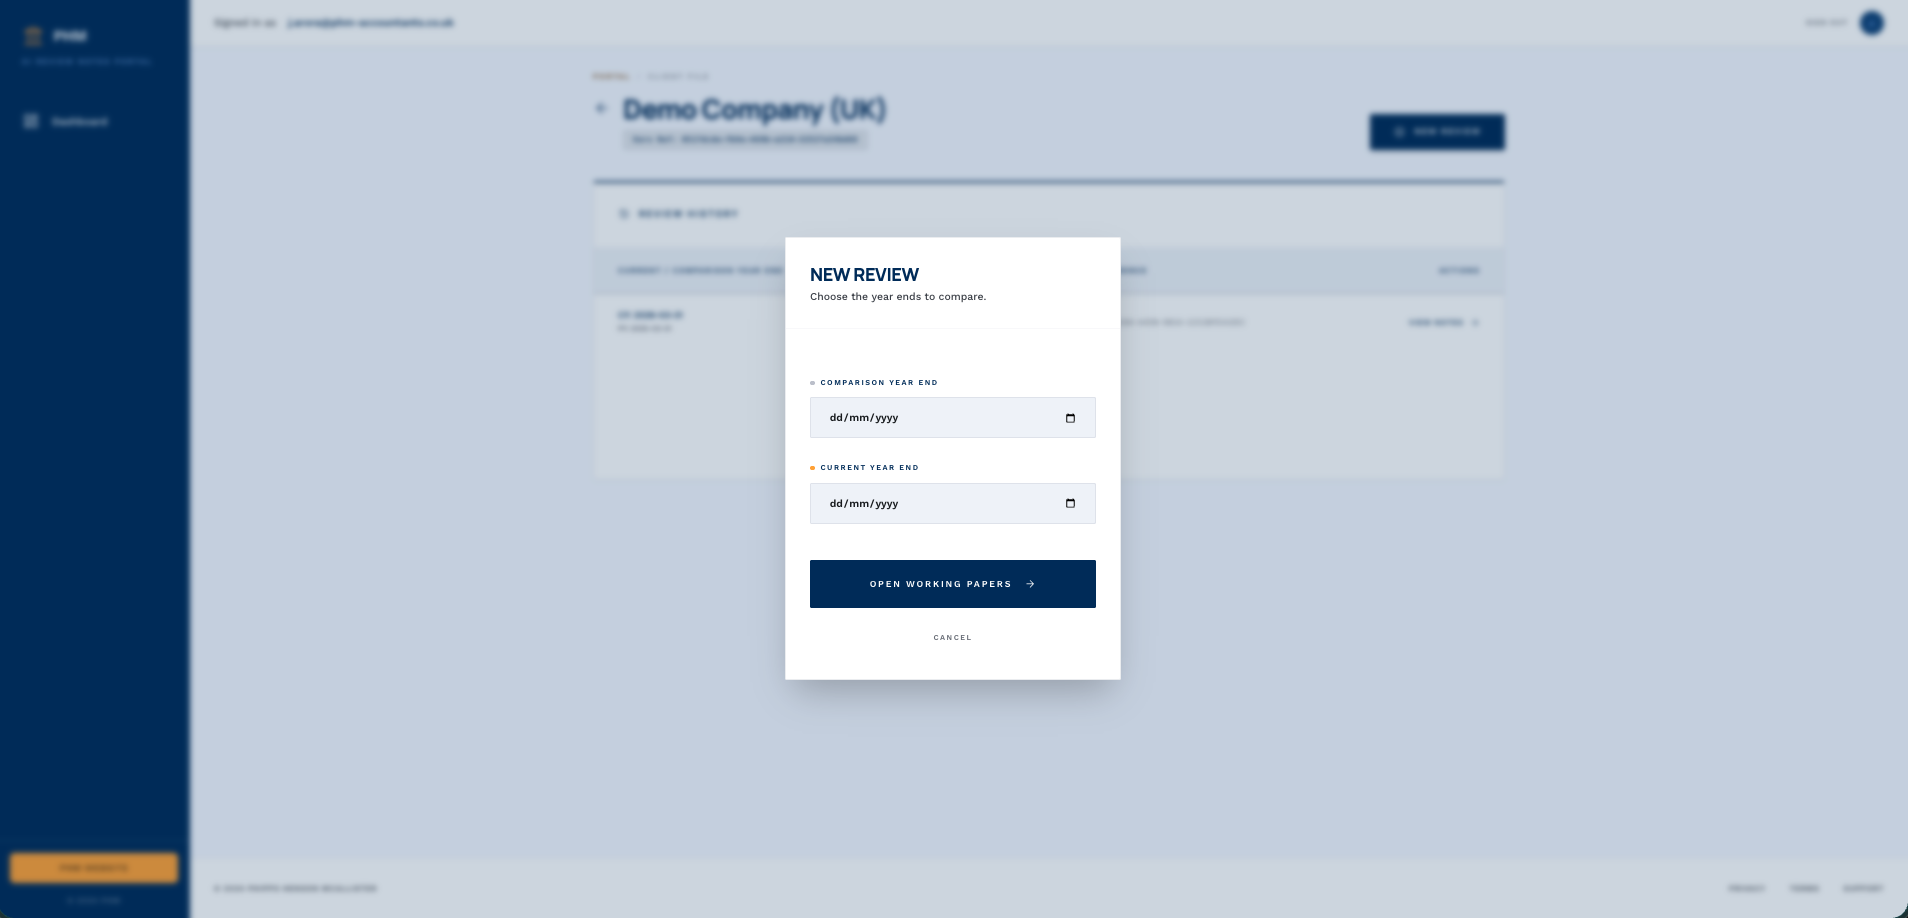
\includegraphics[width=\textwidth]{figures/DATES PAGE}
        \caption{Period Selection Interface}
    \end{subfigure}
    \caption{Supplementary UI Components for Workflow Management}
    \label{fig:supplementary_ui}
\end{figure}

\section{Evaluation Framework: Comparative Analysis of Fine-Tuned Models}
To establish the true capability of modern AI in accounting automation, a comparative evaluation strategy was implemented. Rather than a broad benchmarking of disparate models, this research focuses on the performance of the project's fine-tuned \textbf{GPT-4.1} variants, compared against each other and against the frontier \textbf{GPT-5.4} model using various prompting techniques.

\subsection{Fine-Tuned Model Iterations (GPT-4.1)}
The fine-tuning process was conducted using Azure AI Foundry, specifically targeting the \textbf{GPT-4.1} model---selected for its architectural stability and mature fine-tuning API support. Three distinct fine-tuning recipes were developed using Supervised Fine-Tuning (SFT):
\begin{itemize}
    \item \textbf{FT-A Raw Note SFT:} minimally cleaned historical notes paired with Xero-derived context.
    \item \textbf{FT-B Scrubbed Narrative SFT:} training notes with non-statutory chatter removed so the model learns a tighter accounting narrative.
    \item \textbf{FT-C Scrubbed Plus Rules SFT:} the scrubbed set augmented with deterministic materiality and recurring-subscription cues from the data pipeline.
\end{itemize}

At live benchmark time, the Azure AI Foundry project exposed four callable GPT-4.1 fine-tuned deployments rather than only the three planned recipe labels above. Rather than excluding the extra deployment by hand, all four callable fine-tuned deployments were retained in the measured benchmark so that the comparison reflected the actual project state and did not depend on cherry-picking.

A critical component of this phase was the "Data Scrubbing" pipeline, which was engineered to strip unpredictable human-written narrative (often containing irrelevant "gossip" or non-statutory commentary) from the training corpus. This ensured that the model learned to prioritize mathematical alignment with the Xero Trial Balance over stylistic mimicry of inconsistent human notes.

The training performance was monitored via two primary indicators:
\begin{itemize}
    \item \textbf{Training Loss:} The best run finished with a final train loss of \textbf{1.27}, the second with \textbf{1.36}, and the weakest run with \textbf{1.88}. This spread matters because it shows the fine-tuning process was not uniformly successful across all runs.
    \item \textbf{Mean Token Accuracy:} The corresponding final mean token accuracies were \textbf{0.69}, \textbf{0.67}, and \textbf{0.60}. In practical terms, the first two runs converged into the expected accounting-note range, while the third lagged and later aligned with the weaker behaviours observed in live generation.
\end{itemize}

\begin{figure}[H]
    \centering
    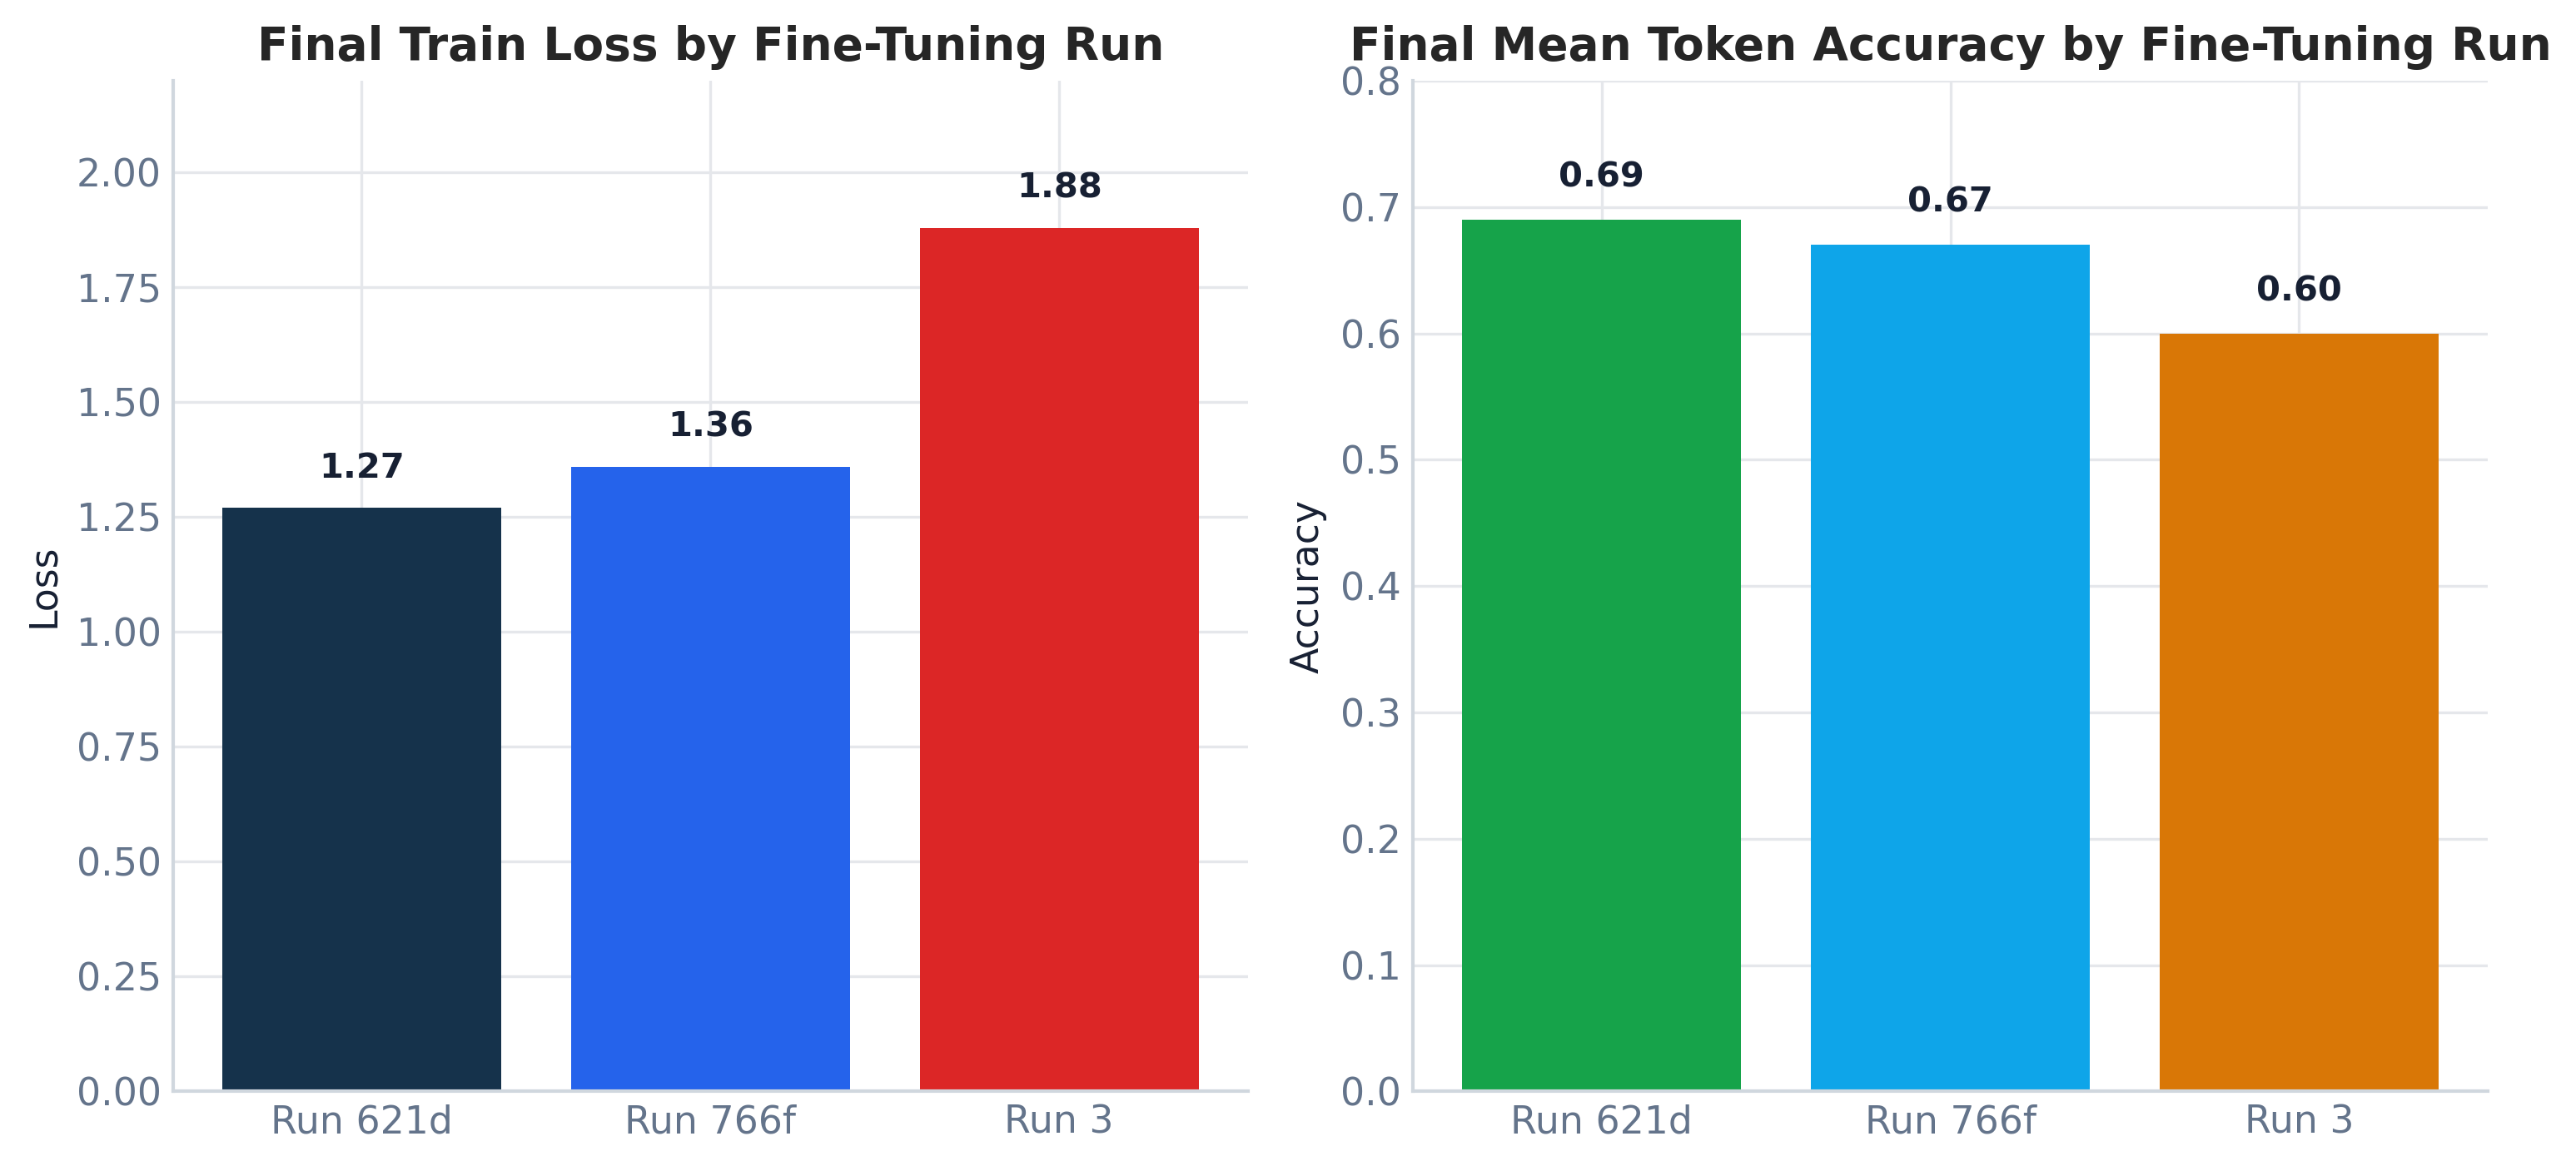
\includegraphics[width=0.9\textwidth]{figures/finetune_run_summary}
    \caption{Final Loss and Mean Token Accuracy Across the Three Main Fine-Tuning Runs}
    \label{fig:training_performance}
\end{figure}

Figure \ref{fig:training_performance} gives the high-level comparison, but the Azure AI Foundry monitor screenshots are also useful because they show the different run shapes directly rather than only the final numbers.

\begin{figure}[H]
    \centering
    \begin{subfigure}[b]{0.32\textwidth}
        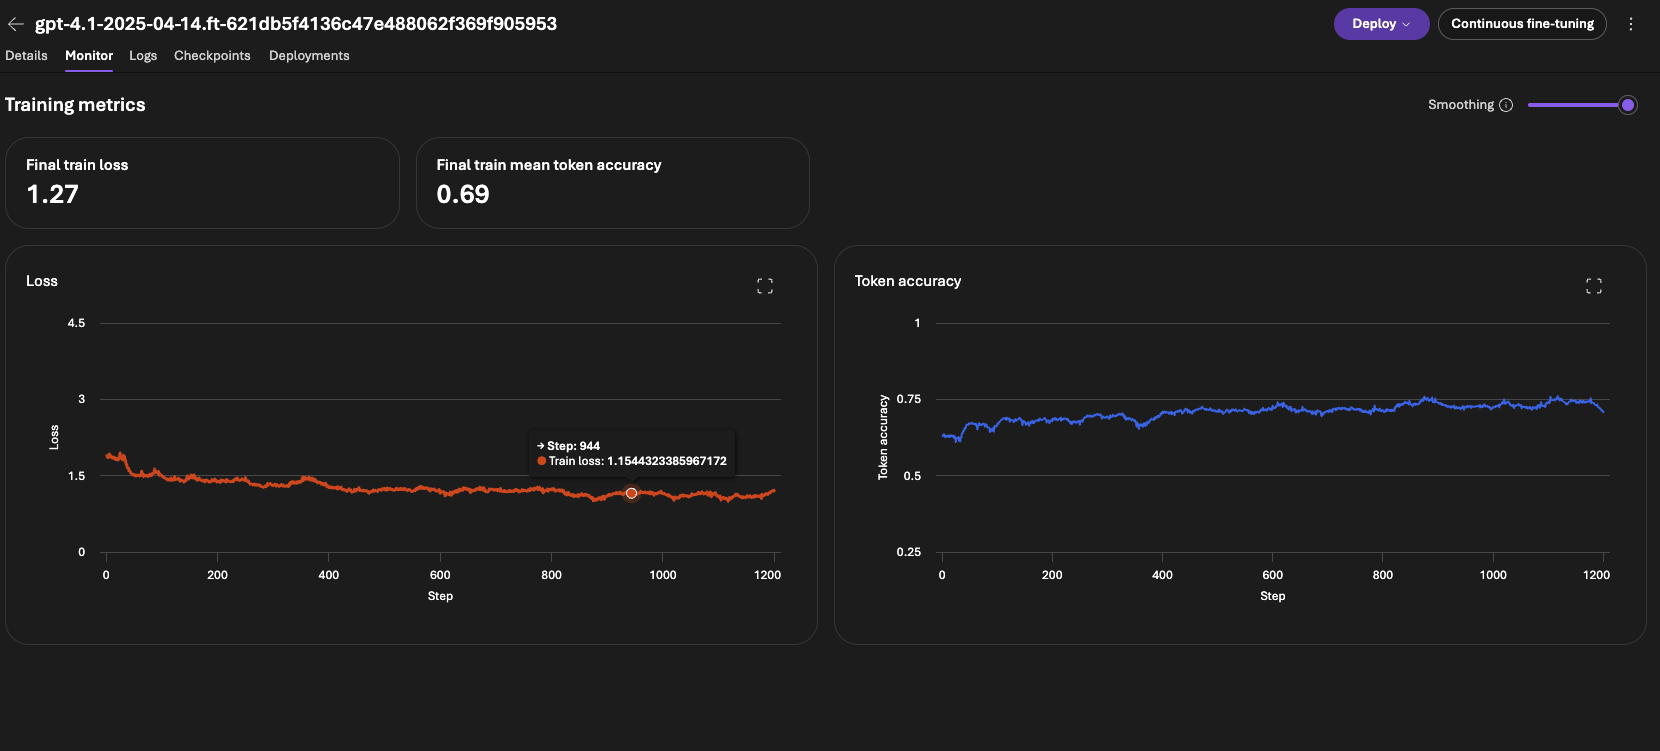
\includegraphics[width=\textwidth]{figures/ft_run_621d_monitor}
        \caption{Run 621d: strongest convergence}
        \label{fig:ft_run_621d_monitor}
    \end{subfigure}
    \hfill
    \begin{subfigure}[b]{0.32\textwidth}
        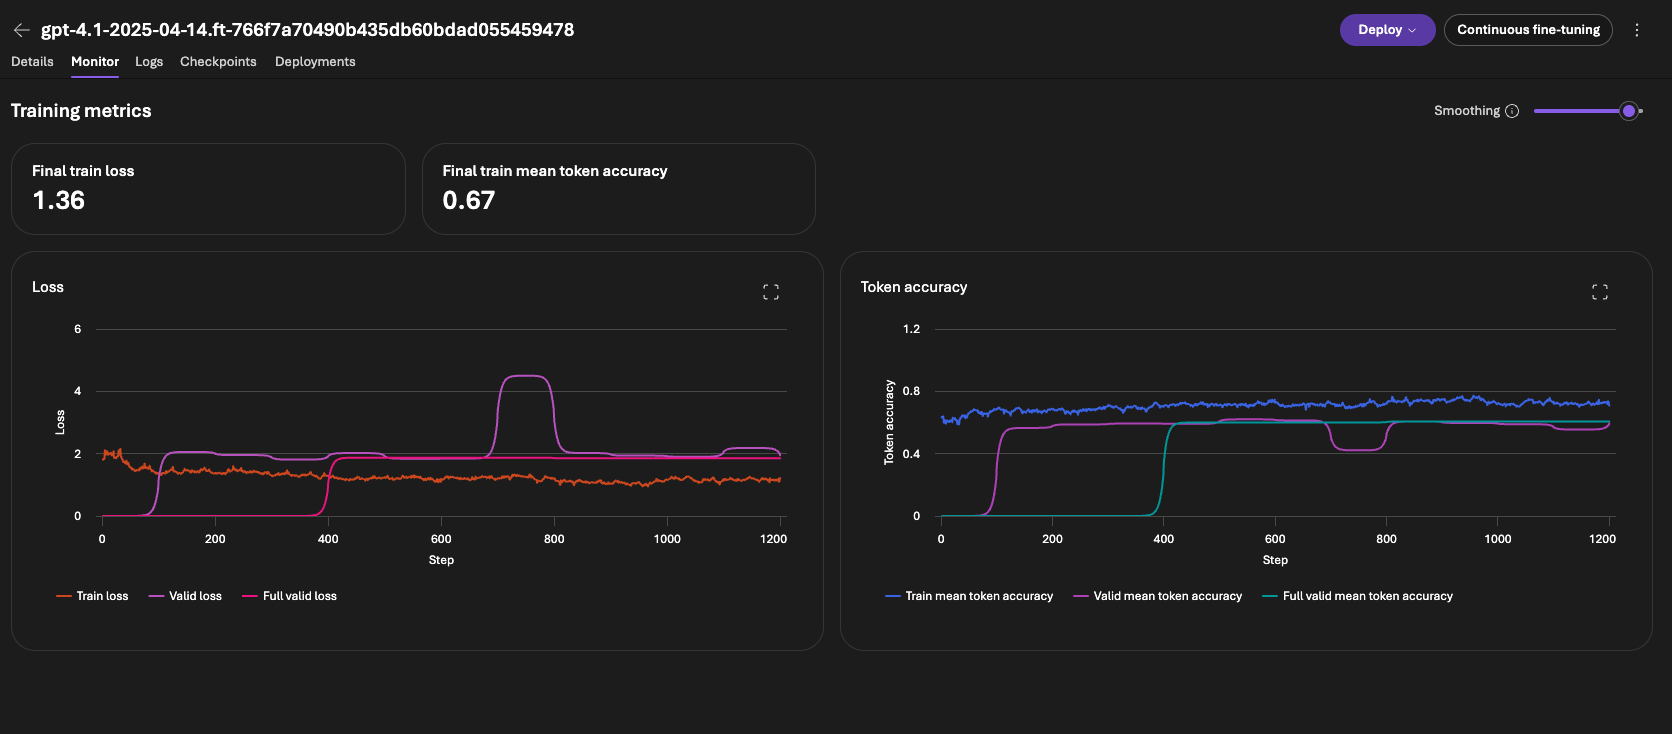
\includegraphics[width=\textwidth]{figures/ft_run_766f_monitor}
        \caption{Run 766f: acceptable but noisier}
        \label{fig:ft_run_766f_monitor}
    \end{subfigure}
    \hfill
    \begin{subfigure}[b]{0.32\textwidth}
        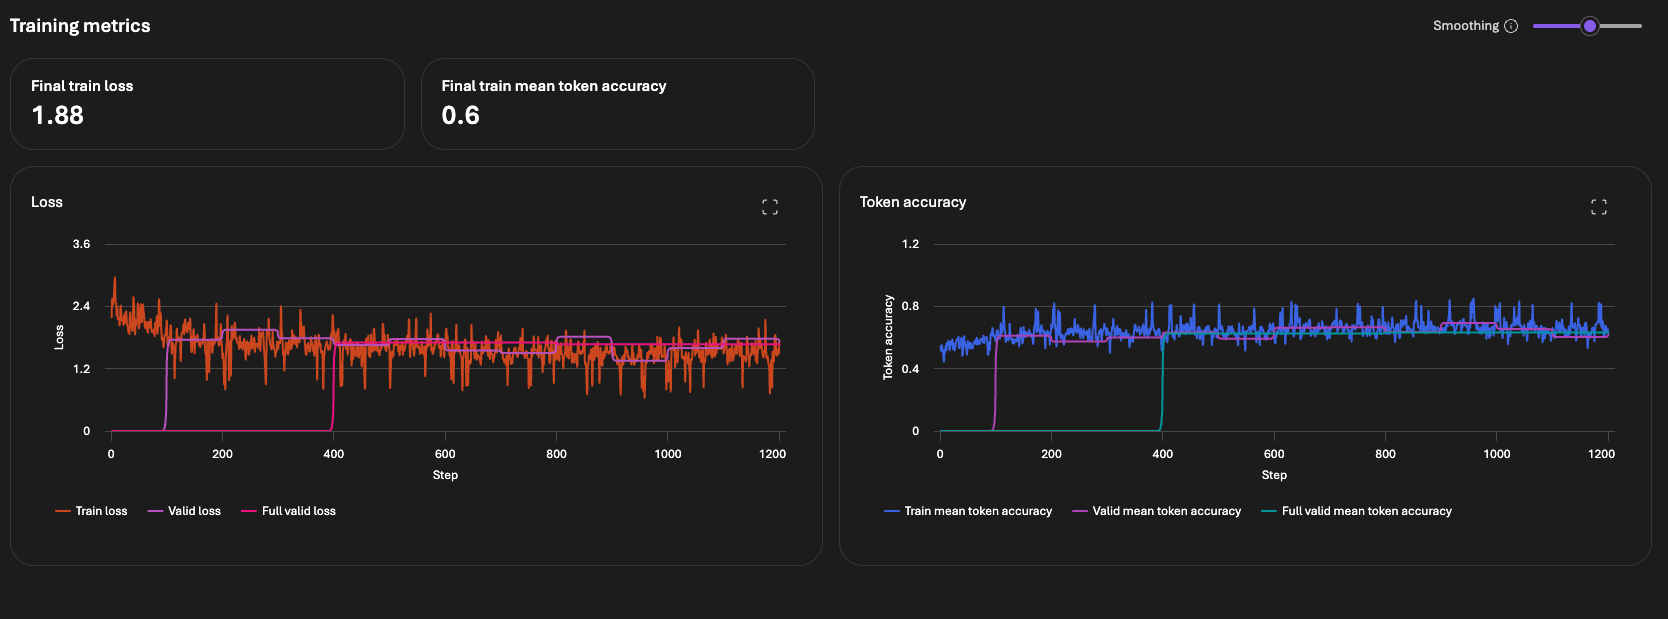
\includegraphics[width=\textwidth]{figures/ft_run_third_monitor}
        \caption{Run 3: weaker convergence}
        \label{fig:ft_run_third_monitor}
    \end{subfigure}
    \caption{Azure AI Foundry Monitor Views for the Three Main Fine-Tuning Runs}
    \label{fig:training_monitor_screens}
\end{figure}

The Foundry monitor views make the quality difference easier to read. The 621d run converged most cleanly and achieved the best final metrics. The 766f run was still usable, but its validation curves were visibly noisier. The third run showed the weakest final loss and token-accuracy values, which is consistent with a poorer checkpoint rather than a mere cosmetic difference in the chart.

These fine-tuned variants are evaluated against each other to identify which training approach best balances narrative precision, numeric fidelity, and reviewer usefulness.


\subsection{Comparative Baseline: Prompt Engineering (GPT-5.4)}
As a high-performance control, the best-performing fine-tuned models are compared against the \textbf{GPT-5.4} model deployed through the Azure AI project endpoint. This baseline model is tested using three primary prompting methodologies to assess whether advanced prompt engineering on a newer model generation can match or exceed the performance of a task-specific fine-tuned predecessor:
\begin{enumerate}
    \item \textbf{Zero-Shot Prompting:} The GPT-5.4 model is given direct instructions without examples.
    \item \textbf{Single-Shot Prompting:} The model is provided with one high-quality example of a standard review note.
    \item \textbf{Few-Shot Prompting:} The model is provided with multiple examples of varying complexity.
\end{enumerate}

The broader validation design uses the 85-record exceptional validation corpus. For the live benchmark reported in this dissertation, a representative three-case subset was executed across the three prompting conditions and all four callable fine-tuned deployments, producing 21 measured generations. The selected cases were chosen to cover a CITB liability adjustment query (\texttt{val\_064}), mixed growth and compliance commentary (\texttt{val\_079}), and unresolved share-issue paperwork (\texttt{val\_084}). Each run was executed with \texttt{temperature=0} and scored against the same accountant-written gold note to isolate the contribution of prompt context from the underlying model capability.

\begin{figure}[H]
    \centering
    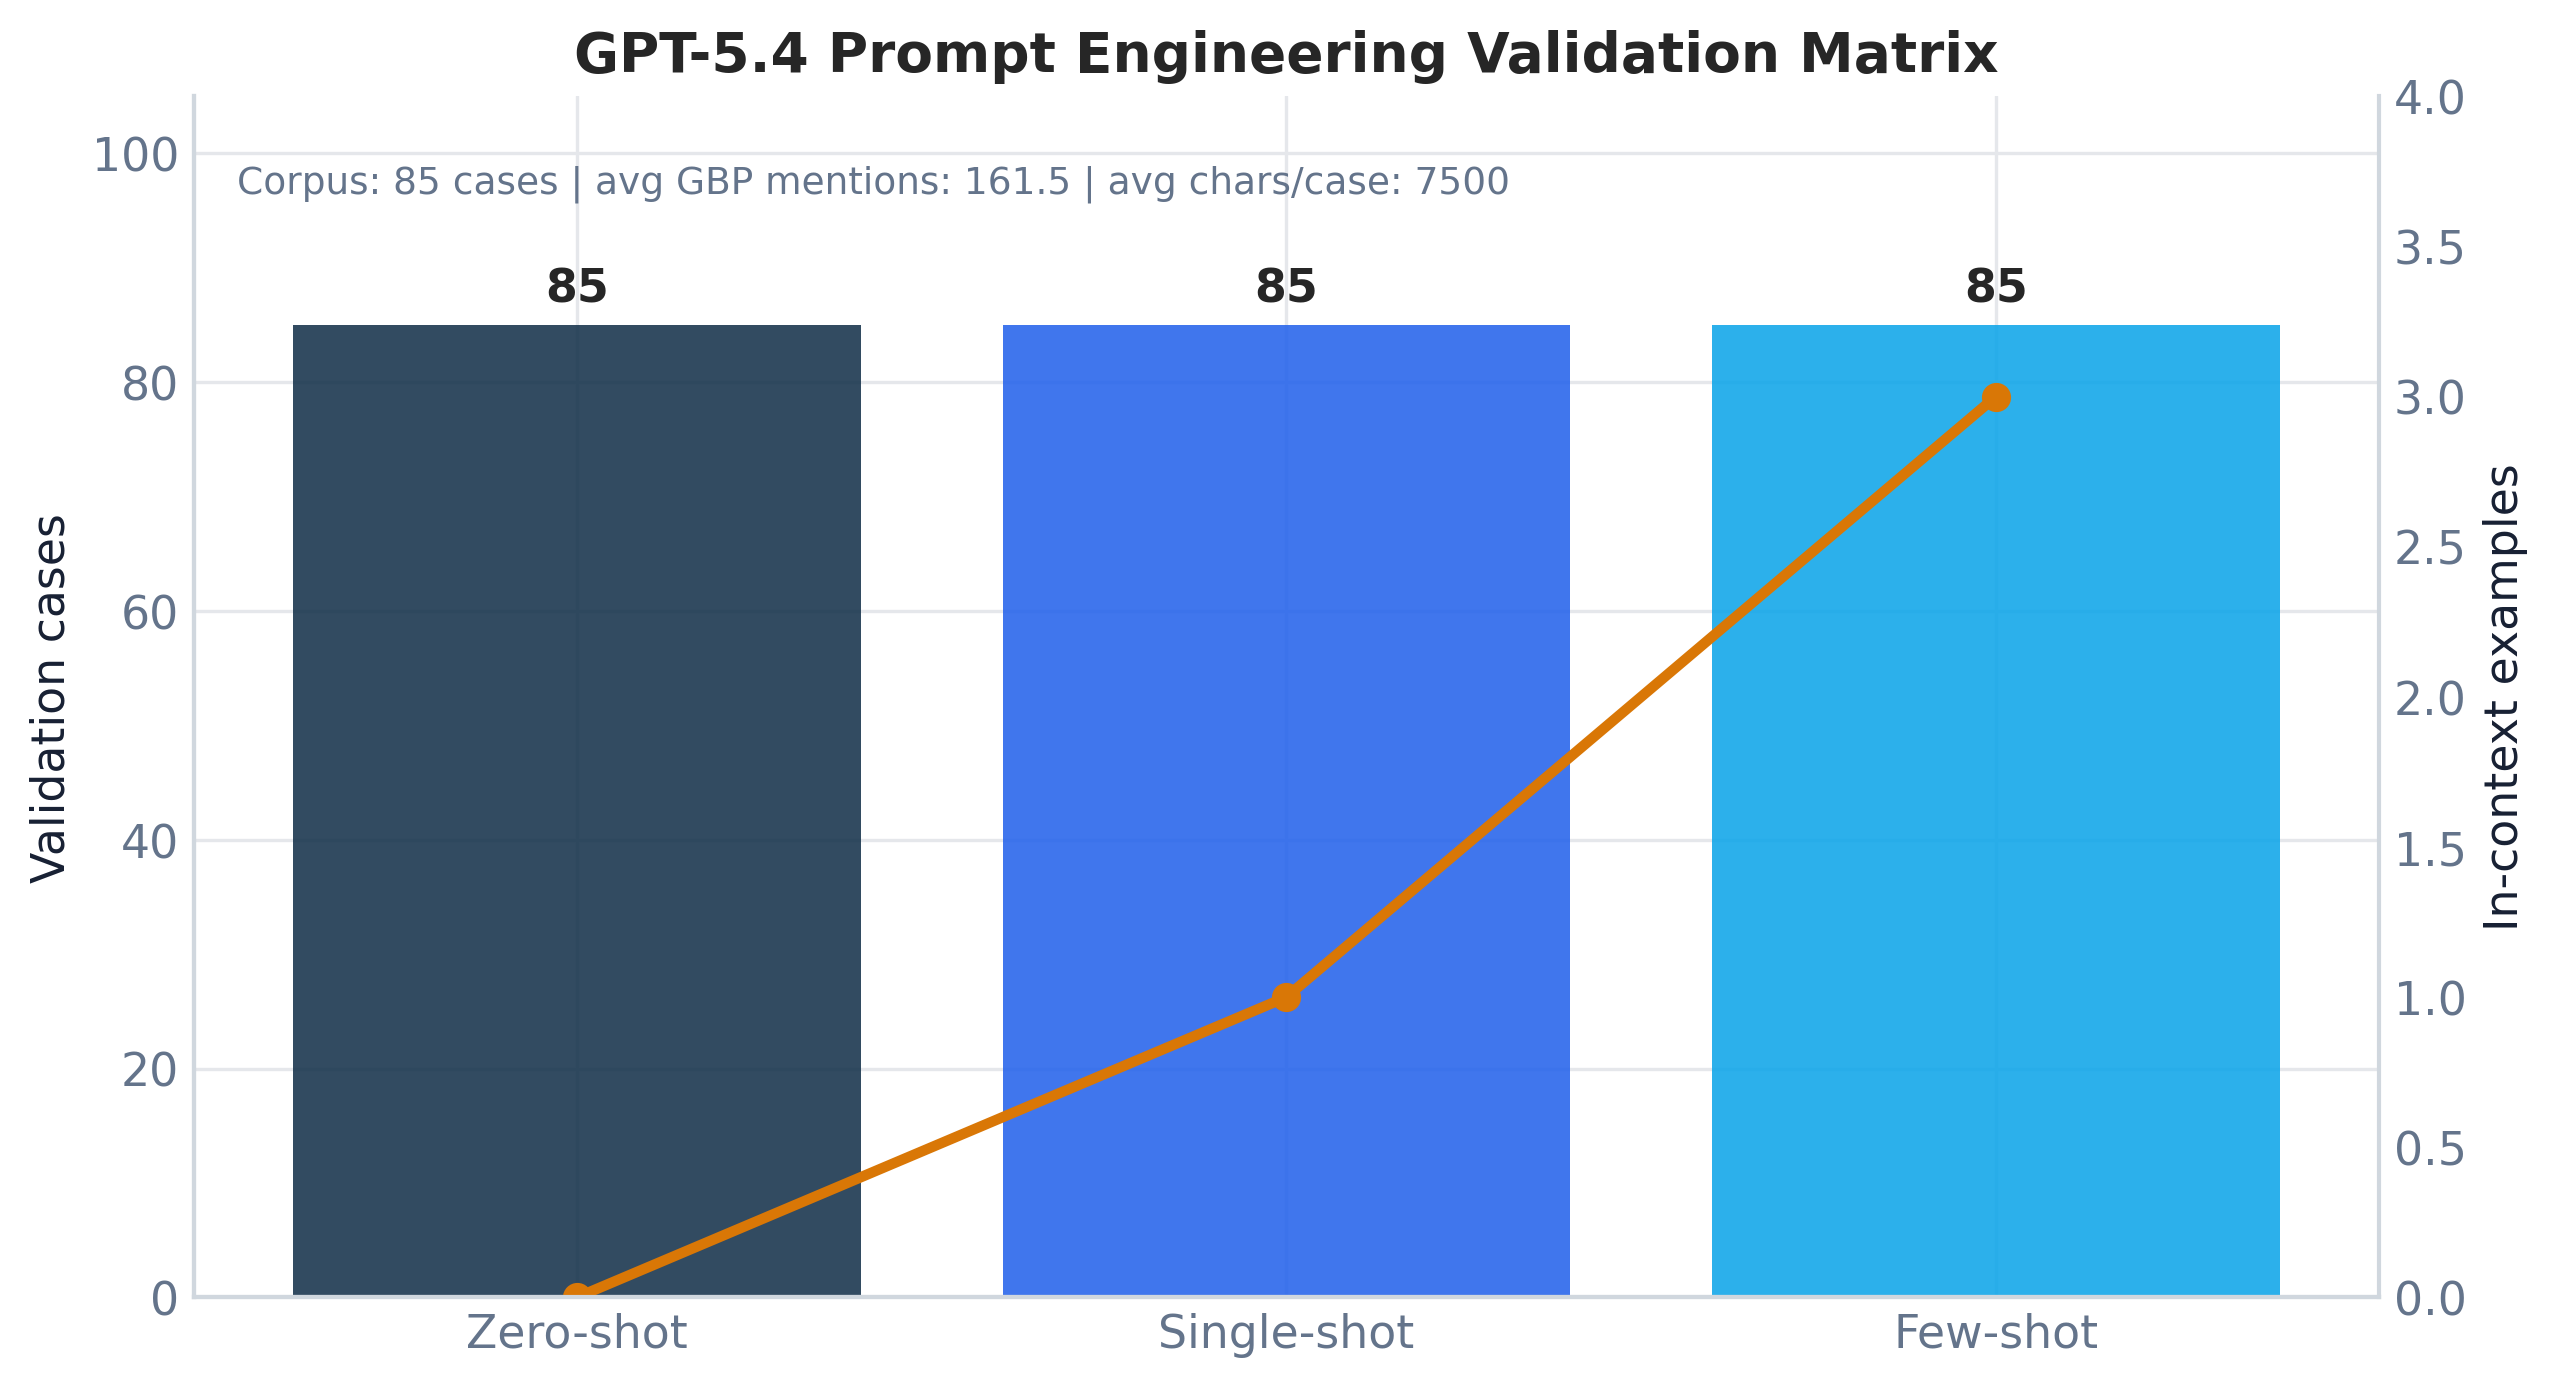
\includegraphics[width=0.82\textwidth]{figures/prompt_engineering_validation_matrix}
    \caption{GPT-5.4 Prompt Engineering Validation Matrix}
    \label{fig:prompt_engineering_validation_matrix}
\end{figure}

The dissertation examples reviewed in the supporting materials do not discuss evaluation only in abstract metric terms. They tie the metric design back to the kinds of cases that matter in professional review. The same approach is used here. The prompt-engineering benchmark is built around long-form accounting cases containing directors' loan accounts, compliance spend, payroll-sensitive commentary, and share issue uncertainty.

\begin{figure}[H]
    \centering
    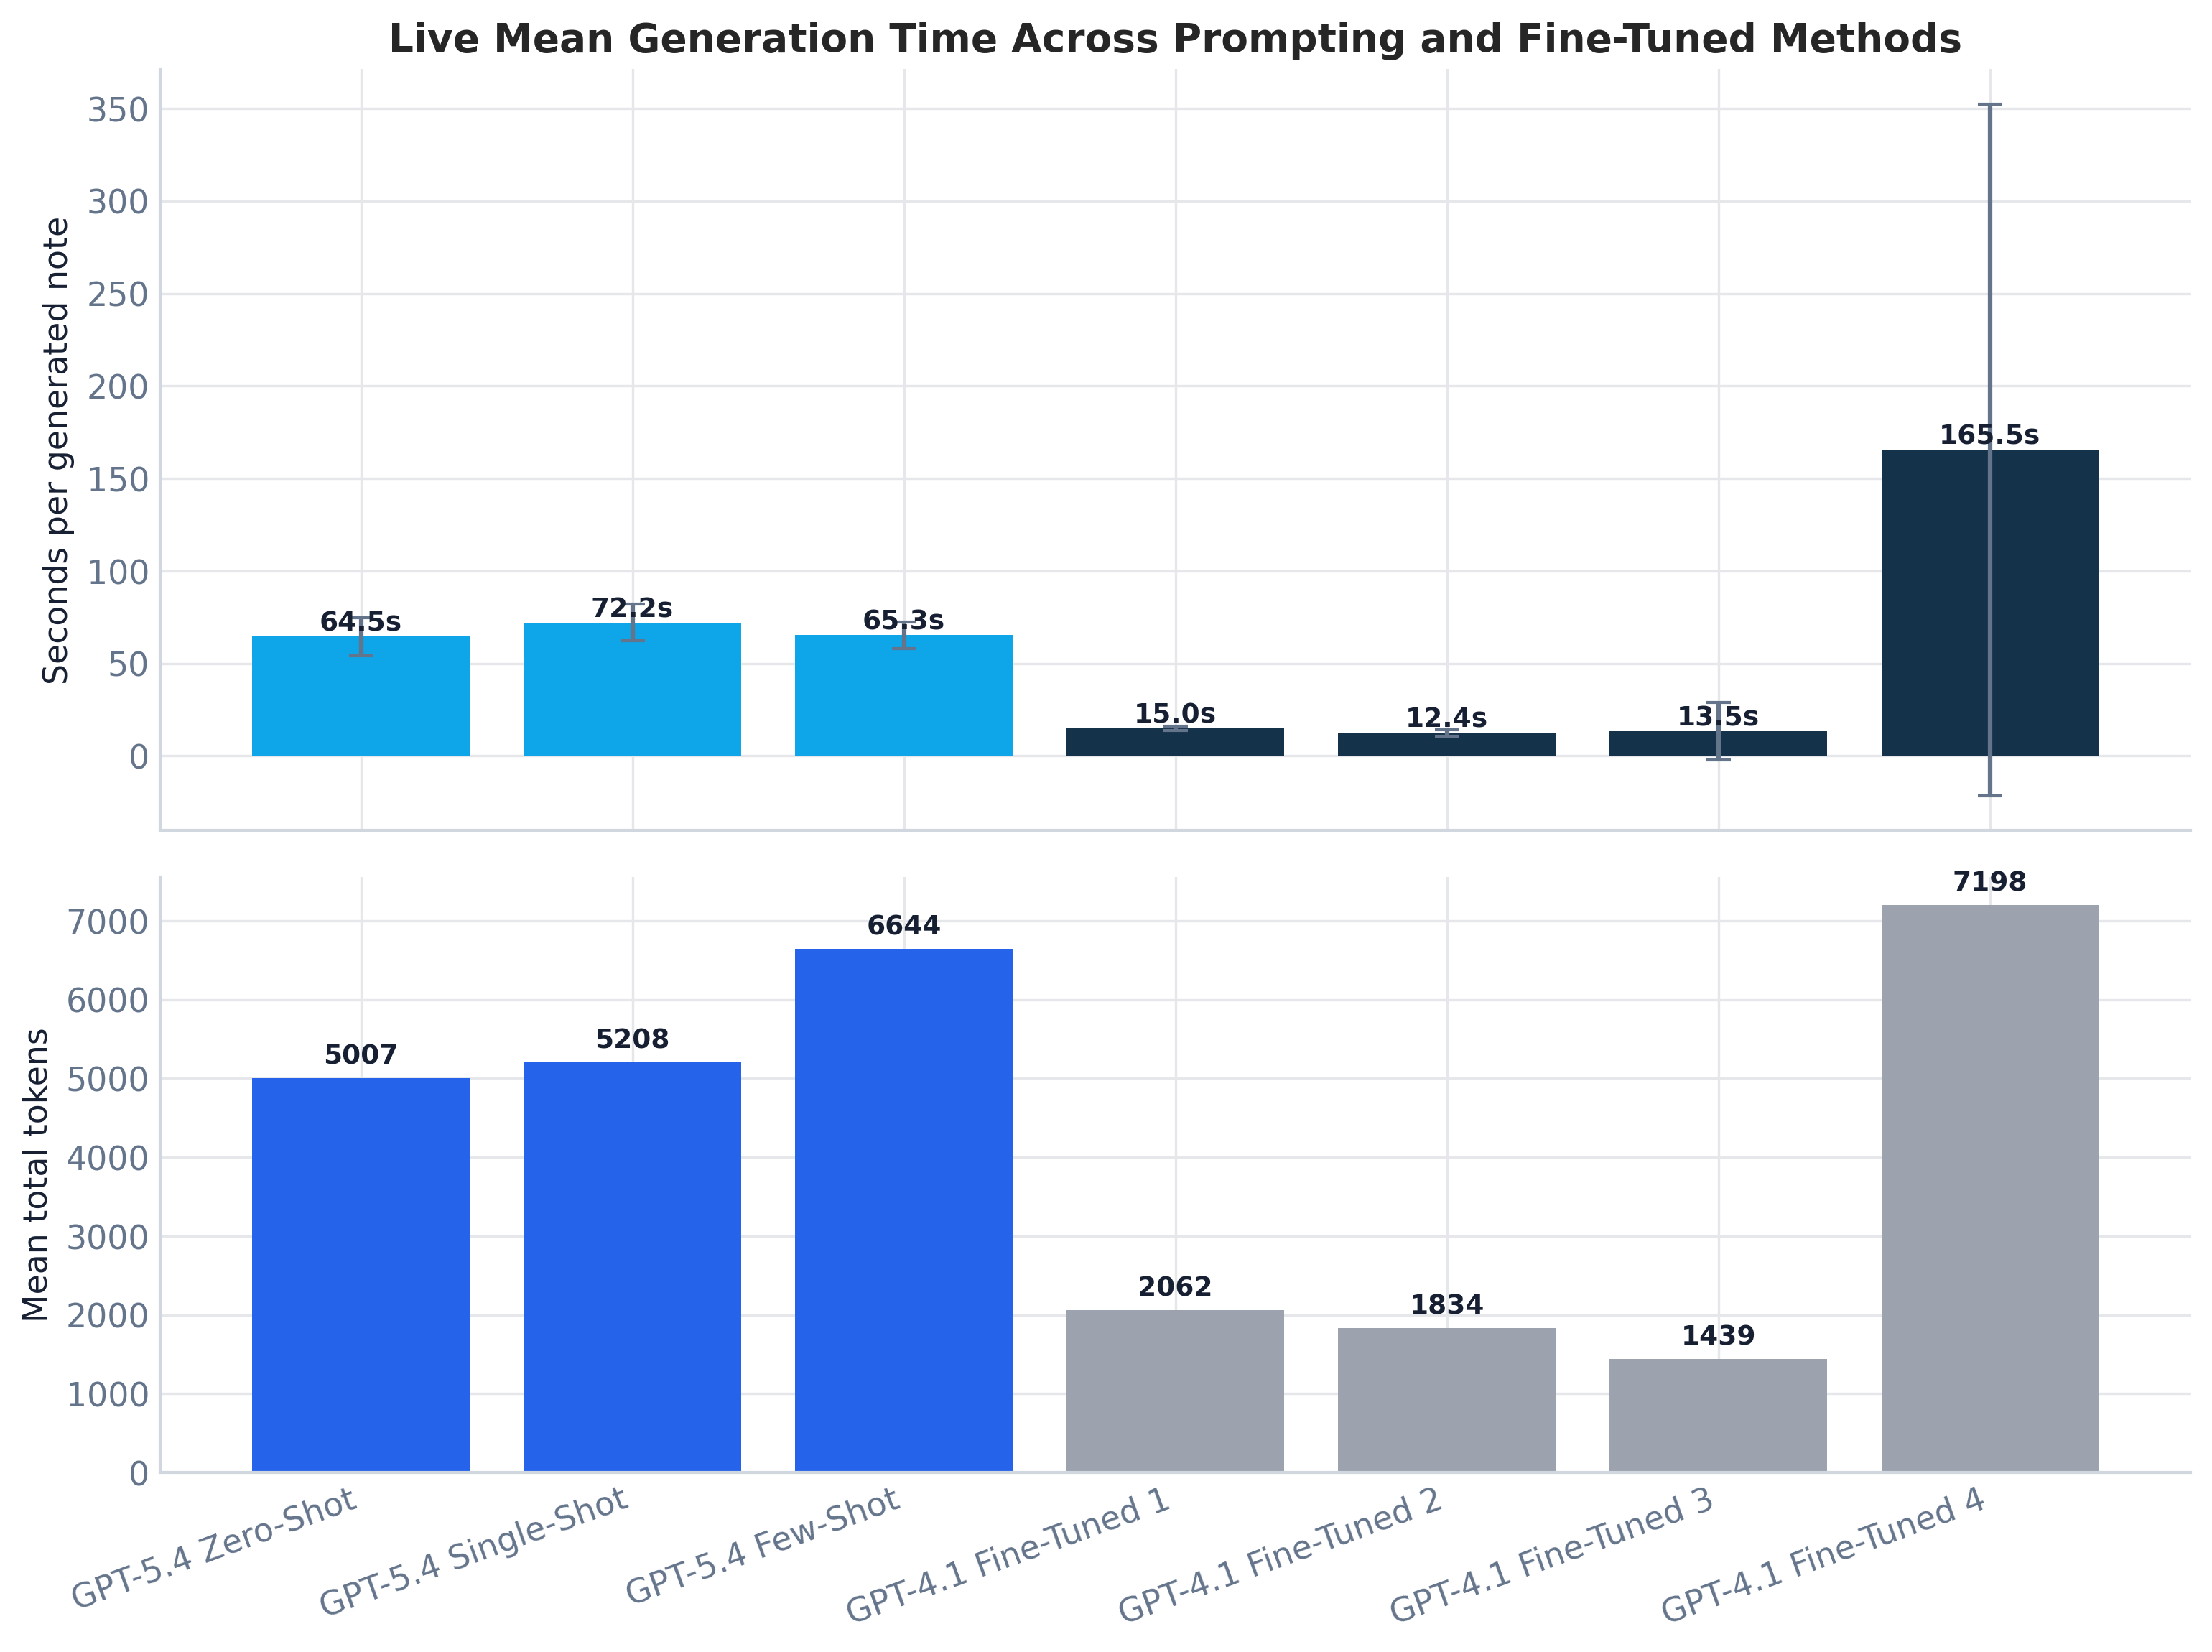
\includegraphics[width=0.9\textwidth]{figures/method_timing_comparison}
    \caption{Measured Time to Produce a Result Across All Tested Methods}
    \label{fig:method_timing_comparison}
\end{figure}

Figure \ref{fig:method_timing_comparison} adds the operational view that the written examples in the context dissertations handled well: the best method is not only the one that writes the cleanest note, but the one that reaches a usable note in a practical amount of time. In the live subset, the prompt-engineering baselines averaged 64.5s (zero-shot), 72.2s (single-shot), and 65.3s (few-shot), while the fastest stable fine-tuned variants averaged 12.4s and 15.0s. The fourth fine-tuned deployment was materially less stable, averaging 165.5s because one case expanded to the output ceiling. That instability is part of the result rather than something to hide.

\subsection{Evaluation Metrics}
All model variations (fine-tuned and prompt-engineered) are tested against four primary criteria:
\begin{itemize}
    \item \textbf{Numeric Fidelity:} Does the generated narrative perfectly match the decimal values extracted from Xero? In financial reporting, a single hallucinated digit constitutes a critical failure.
    \item \textbf{Groundedness and Provenance:} Can the generated statements be traced back to the specific ledger codes provided in the prompt? This measures the system's "Explainability."
    \item \textbf{Narrative Constraints:} Does the model successfully adhere to the firm's strict stylistic rules (e.g., "You" perspective, statutory sequencing, and avoiding redundant journal references)?
    \item \textbf{Time to Produce a Result:} How long each method takes to return a draft note once the case is submitted, together with prompt and completion token usage.
\end{itemize}
The subsequent chapters will detail the specific training datasets used for the fine-tuned models, present the timing profile for all seven tested methods, and compare redacted response examples side by side.
